%\documentclass[12pt,a4paper]{report}
\documentclass[12pt]{report}
\usepackage[right=1.125in, left=1.125in, top=1.125in, bottom=0.815in]{geometry}
%\usepackage{geometry}
\usepackage[dvipsnames]{xcolor}
\usepackage{pdflscape}
\usepackage{setspace}
\usepackage[utf8]{inputenc}
\usepackage{amsmath}
\usepackage{amsfonts}
\usepackage{standalone}
\usepackage{amssymb}
\usepackage{mathtools}
\usepackage{listings}
\usepackage{hyperref}
\usepackage{pgfgantt}
\usepackage{rotating}
\usepackage{bm}
\usepackage{bbm}
\usepackage{lipsum}
\usepackage{pifont}
\usepackage{float}
%\usepackage{color}

\usepackage{graphicx}
\usepackage{subfig}
\usepackage[]{algorithm}
\usepackage{algorithmic}
\usepackage{array}
\usepackage{makeidx}
\newcolumntype{A}{>{\centering\arraybackslash}m{1.8cm}}
\newcolumntype{B}{>{\centering\arraybackslash}m{3cm}}
\newcolumntype{C}{>{\centering\arraybackslash}m{4cm}}
\newcolumntype{D}{>{\centering\arraybackslash}m{2.0cm}}
\newcolumntype{L}{>{\arraybackslash}m{8cm}}
\usepackage[version=3]{mhchem} % Package for chemical equation typesetting \ce{}
\usepackage{siunitx} % Provides the \SI{}{} and \si{} and \num{}
\usepackage[normalem]{ulem}  % stike-through by \sout{}
\usepackage{tikz}
\usetikzlibrary{matrix,arrows,decorations.markings,bending,positioning}
\usepackage{ifthen}
\usepackage{pgf}
\pgfmathsetseed{\number\pdfrandomseed}


% UT diss template setup
\usepackage{utdiss2}
\usepackage[T1]{fontenc}
\usepackage{titlesec, blindtext, color}
\definecolor{gray75}{gray}{0.75}
\newcommand{\hsp}{\hspace{20pt}}

\author{William Ladd Gurecky}
\address{9905 Chukar Circle\\ Austin, Texas 78758}
\title{A CFD-Informed Model for Subchannel Resolution \\ Crud Prediction}
\supervisor{Derek Haas}
\committeemembers
[Benjamin Leibowicz]
[Sheldon Landsberger]
[Kevin Clarno]
{Stuart Slattery}

\previousdegrees{}
% \previousdegrees{, B.S.M.E., M.S.E.}

% image paths
\graphicspath{{../proposal/}{./}{./figs/crud}}

%===========================CUSTOM CMDS=======================================%
\DeclareMathOperator*{\E}{\mathbb{E}}
\newcommand{\xmark}{\ding{55}}%
\makeindex

\begin{document}
\copyrightpage          % Produces the copyright page.
\commcertpage           % Produces the Committee Certification
\titlepage              % Produces the title page.
	
\renewcommand{\thepage}{\roman{page}}
%=================================TITLE=======================================%
%-----------------------------------------------------------------------------%
%! TEX root = ../dissertation_gurecky.tex

% Title.tex
% Author: William Gurecky
% Info:  Title page, table of contents
% Changlog:

%-----------------------------------------------------------------------------%
%\clearpage
%\vspace*{\fill}
%\thispagestyle{empty} % suppress showing of page number
%\doublespacing
%\begin{center}
%Copyright \\

%by \\

%William Ladd Gurecky \\

%2018 \\
%\end{center}
%\singlespacing
%\vspace*{\fill}
%\pagebreak

%-----------------------------------------------------------------------------%
%\begin{titlepage}
%	\centering
%	{\scshape\LARGE The University of Texas at Austin \par}
%	\vspace{1cm}
%	{\scshape\Large Nuclear \& Radiation Engineering \par}
%	\vspace{1.5cm}
%	
%	        {\huge\bfseries Draft \par}
%	{\large\bfseries A CFD-Informed Model for Improving Subchannel Resolution Crud Prediction \par}
%
%	\vspace{2cm}
%	{\Large William Ladd Gurecky \par}
%	\vfill

%	\begin{flushright}
%	Dissertation Committee \par
%	\bigskip
%	Dr.~Derek \textsc{Haas}, Supervisor \par
%	Dr. Sheldon Landsberger \par
%	Dr. Benjamin Leibowicz \par
%	Dr. Kevin Clarno \par
%	Dr. Stuart Slattery \par
%	\end{flushright}
%	\vfill
%	{\large \today\par}
%\end{titlepage}
%%-----------------------------------------------------------------------------%
%\pagebreak


%-----------------------------------------------------------------------------%
\clearpage
\vspace*{\fill}
\thispagestyle{empty} % suppress showing of page number
\begin{center}
%\begin{quotation}
\em % optional -- to switch to emphasis (italics) mode
To family and friends
%\end{quotation}
\end{center}
\vspace*{\fill}

\pagebreak



%! TEX root = ../dissertation_gurecky.tex

%\section*{Acknowledgments}
%\addcontentsline{toc}{chapter}{Acknowledgments}
\acknowledgments

I would like to acknowledge Dr.~Kevin Clarno, Dr.~Stuart Slattery, Dr.~Derek Haas, Dr.~Sheldon Landsberger, Dr.~Ben Leibowicz and Dr.~Robert Salko for their technical guidance and general advice throughout my graduate studies.

Special thanks to Dr.~Erich Schneider who fostered many a students' interest in nuclear engineering \& software development, including mine.

This research was supported by and performed in conjunction with the Consortium for Advanced Simulation of Light Water Reactors (http://www.casl.gov), an Energy Innovation Hub (http://www.energy.gov/hubs) for Modeling and Simulation of Nuclear Reactors under U.S. Department of Energy Contract No. DE-AC05-00OR22725.
\newpage


%Do we want the abstract? 
%\input{./sections/abstract.tex}

\pagebreak
\tableofcontents
\pagebreak

%-----------------------------------------------------------------------------%
%! TEX root = ../dissertation_gurecky.tex

% acryn.tex
% Author: William Gurecky
% Info:  Acronyms
% Changlog:

%-----------------------------------------------------------------------------%
%\section*{Acronyms}
\acronyms
\begin{tabular}{l l}
BHF & Boundary Heat Flux \\
CASL & Consortium for Advanced Simulation of LWRs \\
CDF  & Cumulative Density Function \\
CFD &  Computational Fluid Dynamics \\
CILC & Crud Induced Local Corrosion \\
CIPS & Crud Induced Power Shift \\
CRUD & Chalk River Unidentified Deposit (crud) \\
CTF &  Coolant boiling in rod arrays–Two Fluid (COBRA-TF) \\
FOI &  Field of Interest \\
GBRM & Gradient Boosted Regression Model \\
GBRT & Gradient Boosted Regression Tree \\
HTC  & Convective Heat Transfer Coefficient \\
LANL & Los Alamos National Laboratory \\
LOO & Leave-one-out \\
LOOCV & Leave-one-out cross validation \\
LS  &  Least Squares \\
LWR & Light Water Reactor \\
ML  &  Maximum Likelihood \\
ORNL & Oak Ridge National Laboratory \\
PDF  &  Probability Density Function \\
PWR  & Pressurized Water Reactor \\
ROM &  Reduced Order Model \\
RV  & Random Variable \\
TH  &  Thermal Hydraulic \\
TKE &  Turbulent Kinetic Energy \\
VERA & Virtual Environment for Reactor Applications \\
\end{tabular}

\pagebreak

%-----------------------------------------------------------------------------%
%\section*{Nomenclature}
\nomenclature

\section*{Functions \& Maps}
\begin{tabular}{l l}
$c(\cdot)$ & Copula density function \\
$C(\cdot)$ & Copula cumulative density function \\
$\varphi(\cdot)$ & Copula generator function \\
$f(\cdot)$ & Marginal density function \\
$F(\cdot)$ & Marginal cumulative density function \\
$\mathcal G(\cdot)$ & Crud generator function \\
$h(\cdot)$ & Joint density function \\
$H(\cdot)$ & Joint cumulative density function \\
$\mathcal F(\cdot)_M$ & Gradient boosted model \\
$\mathcal R$ & Mapping from sample space to a location on the rod surface \\
\end{tabular}

\section*{Symbols}
\begin{tabular}{l l}
$t$ & Time \\
$T$ & Temperature \\
$k$ & Turbulent kinetic energy \\
$q''$ & Boundary heat flux \\
$\mathbf p$ & Auxiliary predictive variables \\
$Q_{\tau}$ & Quantile function (inverse CDF) \\
$q_{\tau}$ & The $\tau^{th}$ quantile \\
$\rho_{\tau}$ & Kendall's tau \\
$\theta$ & Marginal distribution parameter \\
$\theta_c$ & Copula shape parameter \\
$\Theta_c$ & Archimedean copula family \\
$\mathbf C$ & Crud state vector \\
$C_m$ & Crud mass density \\
$C_b$ & Crud boron density \\
$C_t$ & Crud thickness \\
$\mathbf X$ & Random vector \\
$X$ & Random variable \\
\end{tabular}


\listoftables
%\addcontentsline{toc}{chapter}{List of Tables}

\listoffigures
%\addcontentsline{toc}{chapter}{List of Figures}

\pagebreak
%-----------------------------------------------------------------------------%


%=================================BODY========================================%
\titleformat{\chapter}[hang]{\Huge\bfseries}{\thechapter\hsp\textcolor{gray75}{|}\hsp}{0pt}{\Huge\bfseries}
\renewcommand{\thepage}{\arabic{page}} % Arabic numerals for page counter
\setcounter{page}{1}
% \onehalfspacing
\doublespacing  % UT formatting spec
%-----------------------------------------------------------------------------%
%
\chapter{Introduction}
\label{chap:intro}
%! TEX root = ../outline.tex

The Consortium for Advanced Simulation of Light Water Reactors (CASL) selected several problems identified by industry partners as critical, inadequately understood, engineering-scale phenomena, which would provide financial and safety benefits to the nuclear power industry if resolved~\cite{Turinsky15}. The problem of interest in this work is the prediction of Chalk River unidentified deposit (crud) growth rates. In an effort to simulate the
effects of crud on the power and burnup distribution, a code produced by a Los Alamos National Laboratory (LANL)
and Oak Ridge National Laboratory (ORNL) collaboration under the name MAMBA was developed  \cite{collins16}.
The development of the MPO Advanced Model for Boron Analysis (MAMBA) and other supporting Virtual Environment for Reactor Applications (VERA) tools provided a starting point for the high-to-low (hi2lo) methods at hand.
\index{CASL} \index{VERA}

A phenomena known as crud-induced power shift (CIPS) is caused by the presence
of elevated \ce{^{10}B} concentrations in the crud layer.  Since crud is preferentially
deposited on the fuel rods in hot regions of the core and \ce{^{10}B} is a strong neutron absorber, the crud buildup leads to a slight shift in
power production toward the bottom of the core under steady-state operation.
Crud induced power shift impacts the burnup distribution over a cycle, reduces shutdown margin,
and is important to account for when computing thermal
margins of the fuel \cite{lange2017}.  The prediction
of CIPS is especially important for older facilities seeking to uprate power
output or extend their operational lifetime.  Additionally, the presence of crud on the rod surface has been shown
to exacerbate local oxide penetration rates of some zirconium alloys \cite{adamson07}.
This is known as crud-induced local corrosion (CILC).  Improvements in crud
simulation techniques ultimately improve the ability to predict the CIPS and
CILC phenomena for a given fuel loading pattern.  If significant CIPS or CILC can be accurately predicted provided a candidate loading pattern, significant cost savings are possible by ensuring the target burnup is not missed due to the presence of excess crud in the core \cite{lange2017}.  Loading patterns that would yield unfavorable crud buildup could be avoided provided an accurate and robust crud prediction capability is available for use in a production environment. \index{Crud} \index{Crud!CILC} \index{Crud!CIPS}

The Virtual Environment for Reactor Applications (VERA) is a key component of
CASL's technical portfolio.  The VERA meta-package integrates a variety of physics
packages and multiphysics coupling options to form a robust reactor simulation
capability.  For multi-cycle depletion computations, VERA relies upon the Michigan Parallel Characteristics Based Transport (MPACT) code, a
2-D/1-D method of characteristics neutronics package, coupled with the subchannel
thermal hydraulics code, Coolant Boiling in Rod Arrays–Two Fluid (CTF).
An integrated crud modeling capability
is provided by MAMBA to address the CIPS challenge problem.
\index{MAMBA}

To reduce computation times, the subchannel TH code discretizes the reactor
domain into large, centimeter scale finite volumes. As a consequence of this
discretization scheme, sub-centimeter scale thermal hydraulic effects of the
spacer grids on crud are averaged over large regions on the fuel rods'
surfaces.  Though small scale phenomena are not explicitly modeled, they are
approximately accounted for in a variety of empirically derived closure
relations.  In effect, a single constant estimate for the mean thermal
hydraulic conditions is obtained in each finite volume. \index{CTF}

\section{Significance and Novelty}

Crud growth is dominated by threshold physics \cite{mongoose17}.  Hot and cold spots
present downstream of spacer grids must be accurately resolved by the hi2lo model to predict the maximum crud
thickness and boron precipitation within the crud layer.

It is challenging to faithfully capture the peaks and valleys in
rod surface temperature and TKE distribution by traditional interpolation
techniques because such a model must guard against smearing out the sharp peaks
present in the spatial distributions.
In the present method we forgo a spatial shape function mapping strategy
for a statistically driven approach that predicts the fractional
area of a rod's surface in excess of some critical temperature but not
precisely where such maxima occur.

\section{Crud Background} 

The buildup of crud results from the deposition of metal particulates and corrosion products entrained in the primary coolant loop of a light water reactor on the exterior surface of the fuel rods.  These impurities arise from erosion and corrosion processes elsewhere in the loop.  Of all the coolant impurities, the largest contributor the initial formation of a crud layer on the outer cladding surface is nickel ferrite.  The initial build up of nickel ferrite may be described by the ordinary differential equation (ODE) shown in equation \ref{eq:crud_nife}.
\index{Crud}

\begin{equation}
\frac{d N_{\mathrm{NiFe},c}}{dt} = (\alpha_{\mathrm{nb}} + \alpha_{b}q''_{b} )N_{\mathrm{NiFe}, \mathrm{cool}} - \gamma_k k
\label{eq:crud_nife}
\end{equation}

Where $N_{\mathrm{NiFe},c}$ is the concentration of nickel ferrite in the crud within a small finite volume on the cladding surface.  $N_{\mathrm{NiFe}, \mathrm{cool}}$ is the concentration of nickel and iron impurities in the coolant.  $\alpha_b$ and $\alpha_{nb}$ represent boiling and non-boiling rate constants respectively.  The boiling component of the boundary heat flux (BHF) on the outer cladding surface is given by $q''_b [W/m^2]$. Note that  $q''_b$ is only non-zero when $T>T_{sat}$. $\gamma_k$ is an erosion multiplier and $k$ is the near-wall local TKE.  Crud typically forms where temperatures are high and where subcooled boiling occurs on the rod surface.
\index{Crud!Formation}

%-----------------------------------------------------------------------------%
\chapter{Theory}
\label{chap:theory}
%! TEX root = ../outline.tex

A review of the solution detail afforded by CFD and subchannel thermal hydraulic codes is provided to begin this section along with consequences of their respective spatial discretization schemes on crud growth.  A simplified method for harnessing CFD results to improve expected-value computation of crud on a given CTF face is provided to introduce the hi2lo strategy.  Next, copula and quantile regression are discussed as a means to model the joint distribution of temperature and TKE on the rod surface.   This is followed by an introduction to the gradient boosting machine learning method used to predict the behavior of the joint distribution as a function of local core conditions.  The Monte Carlo method for estimating the integral required to compute the expected crud value is given.  A review of importance sampling is also provided to provide a means to increase the sampling efficiency of the Monte Carlo integration procedure.
The section culminates in an integration of the copula, quantile regression, and importance sampling routines into a complete algorithm for time dependent crud prediction.

\section{Model Approach}

A fundamental difference between the CFD and CTF computations is the average size of the mesh cells.  In the azimuthal coordinate, CTF decomposes a single rod surface into four patches.  An example top down view of typical CFD and CTF meshes for a single pin are given in figure \ref{fig:cfd_ctf_mesh}.  Though both codes employ a finite volume spatial discretization, CFD can resolve the flow at much smaller length scales.  Additionally, each code employs a different set of closure models to the underlying set of coupled energy, mass, and momentum balances.  In practice these differences lead to large discrepancies in boiling, turbulent mixing, and rod surface temperature predictions between the two codes.
\index{Subchannel} \index{CFD}

\begin{figure}[!htbp]
    \centering
    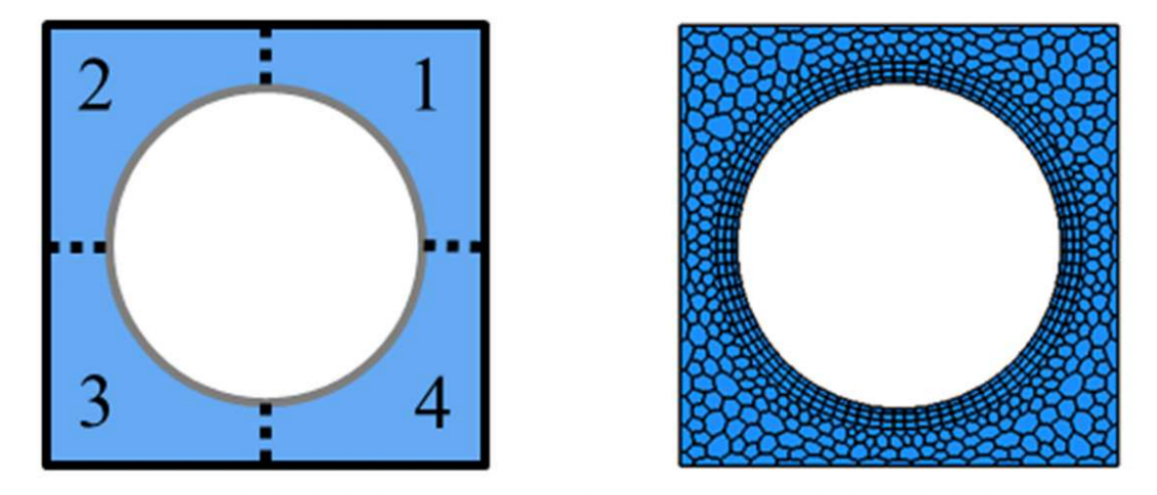
\includegraphics[width=10cm]{../proposal/images/cfd_ctf_mesh.png}
    \caption[Top-down view of typical subchannel and CFD meshes]{Top-down view of typical subchannel (left) and CFD mesh (right) for a single pin \cite{salko12}.}
    \label{fig:cfd_ctf_mesh}
\end{figure}

Shown in figure \ref{fig:model_overview}, on a given CTF rod surface patch, estimates for the surface temperature, TKE, and heat flux are provided as point estimates.  The predicted CTF quantities are an estimate for the average thermal hydraulic conditions over that coarse patch.   Consequently, CTF crud predictions deviate from reality since crud growth is highly sensitive to the presence of subcooled boiling on the rod surface; if CTF predicts a rod surface temperature less than the saturation point in a given patch little or no crud will form when in reality, a small portion of that rod surface could exist above the saturation point and thus harbor crud.  Small localized mistakes in crud predictions compound throughout the core, leading to poor CIPS estimates.

In figure \ref{fig:model_overview}, $f$ denotes a probability density function.  Integration of this density function may be interpreted as computing a fractional area of the rod surface that exists within the specified integration limits.
\begin{figure}[!htbp]
    \centering
    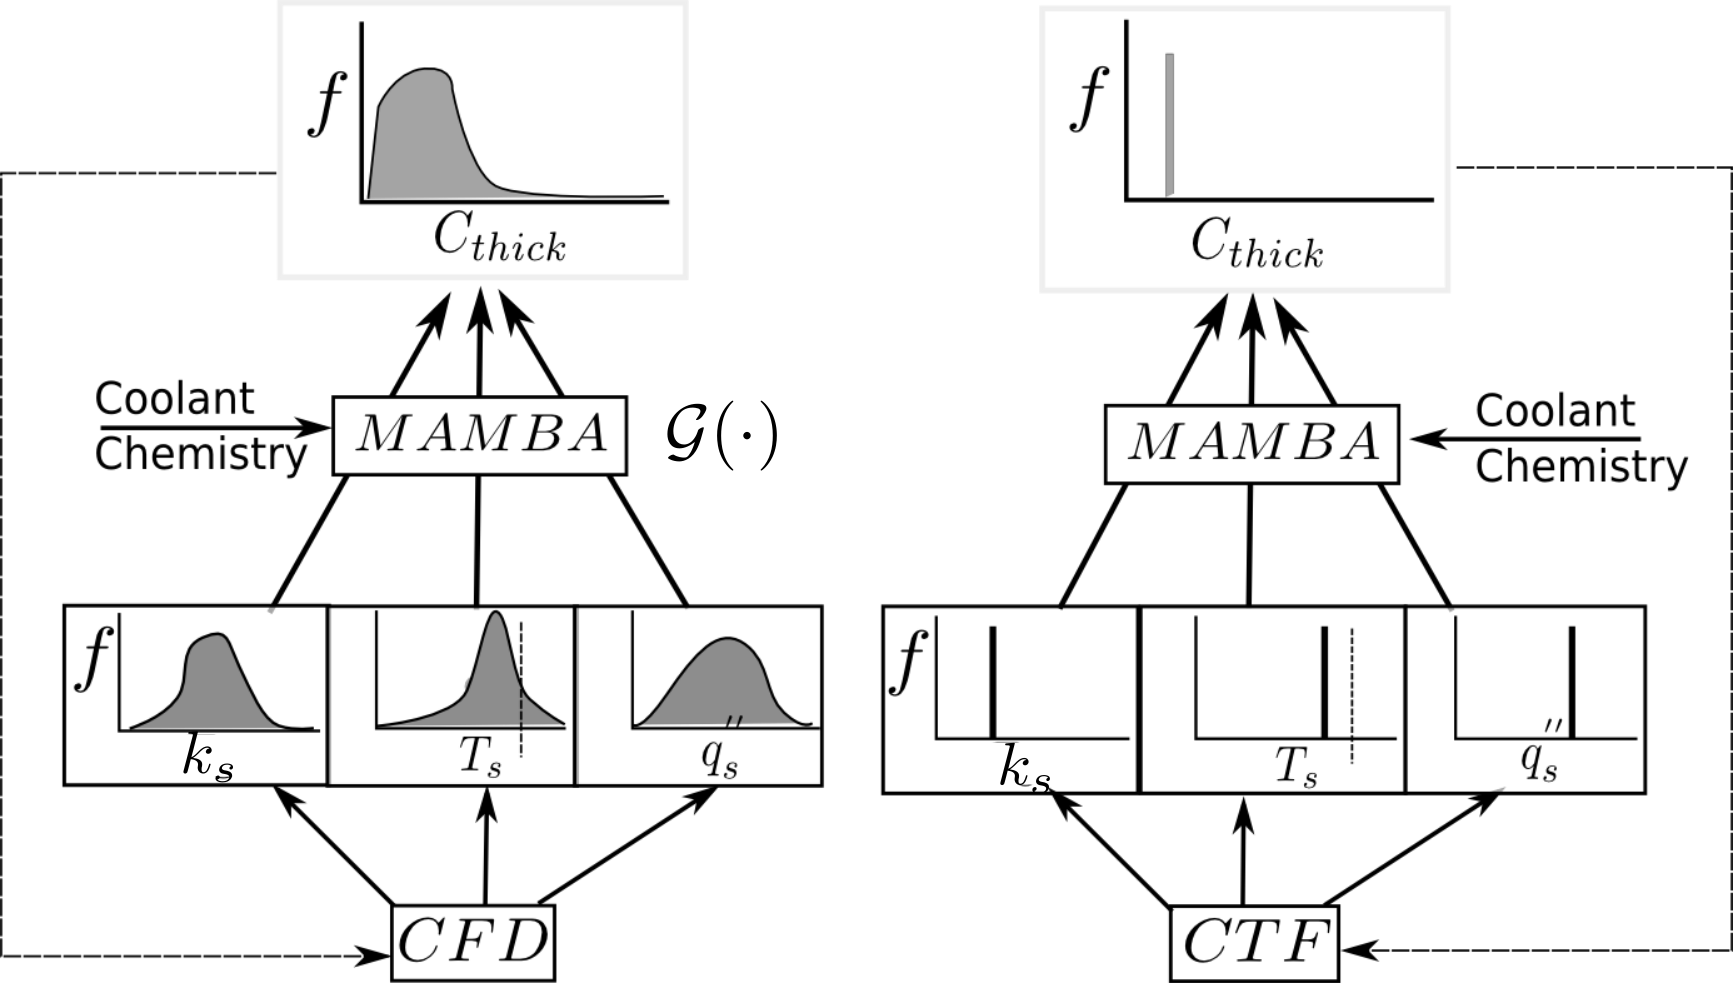
\includegraphics[width=12cm]{figs/theory/model_relations.png}
    \caption{On a single coarse CTF patch: Differences in crud prediction between CFD and CTF models.}
    \label{fig:model_overview}
\end{figure}

CTF estimates mean TH conditions everywhere in the core at a low spatial resolution.  The CFD informed model provides higher order moments about the mean.
\begin{equation}
   \mathbf X(\mathbf p, \mathbf z) = \underbrace{ \bm \mu(\mathbf p, \mathbf{z})}_\text{CTF} +
   \underbrace{\varepsilon({\theta (\bm p, \mathbf z)}) + \bm b(\mathbf p, \mathbf{z})}_\text{CFD Informed}
   \label{eq:hi2lo_overview}
\end{equation}

\begin{itemize}
        \item $\mathbf X$ is a three component vector representing the cladding surface temperature, $T$, turbulent kinetic energy, $k$, and boundary heat flux, $q''$.
        \item $\mathbf z$ denotes spatial coordinates and $\mathbf p$ represents a set of auxiliary predictors.  Auxiliary predictors are covariates that describe local core conditions and may be geometric or thermal hydraulic in nature.
        %Specific auxiliary predictors are introduced in Chapter \ref{sec:ml_cfd}.  Table \ref{tab:features} contains a detailed description of the auxiliary predictive features used in this work.
        \item  $\varepsilon$ is a three-component random vector comprised of temperature, turbulent kinetic energy and boundary heat flux fields.  $\varepsilon$ is distributed according to a CFD informed model with $\theta$ representing free model parameters which are determined from the CFD data.
        \item $\bm b$ is bias between the low and high fidelity models ($\bm \mu_{CTF} - \bm \mu_{CFD}$).  Despite providing identical inlet boundary conditions to both codes bias exists due to algorithmic, closure model and meshing differences between the two codes.
        \item Field averages, $\bm \mu$, are piecewise constant over each CTF patch.
        % \item Note this is a additive model where Salko constructed a multiplicative model.
\end{itemize}

Consider a hypothetical case where the CFD results are normally distributed about the CTF results such that $\varepsilon \sim \mathcal N(0, \bm \Sigma(\mathbf p, \mathbf z))$, where $ \bm \Sigma(\mathbf p, \mathbf z)$ is a covariance matrix that depends on local core conditions.  Shifting the distribution by a constant vector $\bm c=\bm b + \bm \mu_{ctf}$, results in a distribution denoted by $h$ in equation \ref{eq:norm_noise}.
\begin{align}
    \left. h \right|_{(\bm p, \bm z)} & = \mathcal N(\bm c, \bm \Sigma(\mathbf p, \bm z)) \nonumber \\
    & = \left.
        \mathcal N \left(
        \begin{pmatrix}
            c_T \\
            c_k \\
            c_{q''}
        \end{pmatrix}
    ,
        \begin{pmatrix}
            \Sigma_{TT} & \Sigma_{Tk} & \Sigma_{Tq''} \\
            \Sigma_{kT} & \Sigma_{kk} & \Sigma_{kq''} \\
            \Sigma_{q''T} & \Sigma_{q''k} & \Sigma_{q''q''}
        \end{pmatrix}
    \right)
    \right|_{(\mathbf p, \mathbf z)}
\label{eq:norm_noise}
\end{align}
Where $\Sigma_{xx} = \sigma_x^2$ and $\Sigma_{xy} = cov(x,y)$.

Equation \ref{eq:expected_crud} estimates the expected crud mass $C_m$ that accumulates on each CTF patch in time $\delta t$.  Let the CTF face of interest have area $A$.  Let $\mathbf X= \{T, k, q''\}$ denote a random vector of temperature, TKE, and BHF. $\mathbf I$ represents additional known crud parameters, $\mathbf C_o$ is the crud state at the start of the time step.  Let the joint density function of $\bf X$ be denoted by $h$, and it's CDF be denoted by $H$.  The crud model, $\mathcal G(\cdot)$, is common to all CTF faces.  The joint cumulative density's parameters are predicted from the available high resolution CFD data in every CTF face.  In the case of an assumed normal distribution model there are nine unknowns which require fitting:  $\theta = \{ \sigma^2_T, \sigma^2_k, \sigma^2_{q''}, \Sigma_{kT}, \Sigma_{q''T}, \Sigma_{q''k}, c_T, c_k, c_{q''} \}$.  In the subsequent sections we will seek to relax the normality assumption of the CFD residuals about the CTF result.

\begin{align}
        C_m &= A \mu_{m} \nonumber \\
        &= A \E[\mathcal G(\mathbf X|\mathbf C_o, \mathbf I, \delta t)] \nonumber \\
        &= A \iiint \mathcal G(\mathbf X|\mathbf C_o, \mathbf I, \delta t) h(\mathbf X|\theta) d \mathbf X
        \label{eq:expected_crud}
\end{align}

A strategy to compute the unknowns of the joint distribution on each CTF face is required.  The current work proposes a data driven model, $\mathcal F_M$, to predict the unknowns provided a suite of pre-computed CFD results are used to train the machine learning model and local thermal hydraulic conditions provided by CTF at runtime are utilized to evaluate the model on each CTF face. Algorithm \ref{algo:basic_crud_algo} is used to compute the total crud mass in each CTF face.

\begin{algorithm}[H]
    \captionsetup{labelfont={sc,bf}, labelsep=newline}
    \caption{Generic hi2lo method for crud prediction.}
    \begin{algorithmic}[1]
    \STATE \textbf{Initialization}
    \STATE (1) Pre-process training set.
    \STATE $\ \ $   (1b) Fit the joint distribution parameters, $\theta$, to known CFD data. 
    \STATE $\ \ $   (1c) \textbf{def:}  $\ \theta \leftarrow \mathcal F_M(\mathbf p, \mathbf z )$
    \STATE (2) Train model:  $\hat{\mathcal F_M} =  \mathrm{argmin}_{\mathcal F}$
      $\E \left[ L(\mathcal{F}_M (\mathbf p, \mathbf z), \theta) \right]$
\FOR {CTF face, $j$}
    \STATE Evaluate ML model $\hat \theta_j \leftarrow \hat{\mathcal F_M}(\mathbf p_j, \mathbf z_j)$ \;
    \STATE Reconstruct $\hat H_j(\cdot |\hat \theta_j)$ \;
    \STATE Draw samples $\mathbf X \sim \hat H_j$ \;
    \STATE Evaluate equation \ref{eq:expected_crud} via Monte Carlo approximation \;
\ENDFOR
    \end{algorithmic}
\label{algo:basic_crud_algo}
\end{algorithm}
Where $L(\cdot)$ is a generic differentiable loss function.  A discussion on the machine learning model and loss function follows in section \ref{chap:GBRT}.  The reconstruction of the joint density function $\hat H$ from copula and univariate quantile functions is discussed in section \ref{chap:quantiles}.  Monte Carlo and importance sampling are discussed in section \ref{chap:mc_crud}.

Algorithm \ref{algo:basic_crud_algo} may be broken down into five generic components.  \emph{Lines 2-5:} Establish a relationship between the local core geometry and thermal hydraulic conditions to the behavior of surface temperature, TKE and boundary heat flux distributions using a pre-computed suite of CFD results. \emph{Line 7:} The prediction of joint distribution parameters. These parameters will take the form of conditional quantiles and parameters of a copula in the present work. \emph{Line 8:} The reconstruction of the joint temperature, TKE, and boundary heat flux distribution in each CTF face given predictions provided by evaluating the data driven model $\mathcal F_M$ at the local core conditions adjacent to the CTF face under consideration. \emph{Line 9:} Sampling from the reconstructed distribution.  \emph{Line 10:} Integration of the crud density by a Monte Carlo procedure.

% A critical question to answer is:  Can a data driven machine learning model adequately predict the parameters of a probability distribution on each CTF face: $Var[(\hat \theta_j \leftarrow \mathcal M(\mathbf p_{j}, \gamma))] < \epsilon$?  There is some uncertainty in the optimal machine learning model parameters.  This propagates to the distribution parameters which ultimately governs the uncertainty of the crud results.  An adequate model in this context reduces the uncertainty in the final crud estimate to some acceptable level.

% In addition to improving the expected value prediction of crud on each CTF patch vs the CTF standalone case, the model provides the capability to estimate the likelihood of extreme value events i.e. $\mathcal P_f \propto Pr(C_t(x) > C_t^*)$, where $C_t^*$ is some critical crud thickness and $\mathcal P_f$ is a cladding failure probability.  This would be difficult to quantify with CTF/MAMBA alone and requires either a hi2lo approach or detailed investigation of at-risk pins with high fidelity CFD computations.  A significant challenge is computing an estimate for $Var(\mathcal P_f) = \E[(\mathcal P_f - \E(\mathcal P_f))^2]$, or similarly, the variance in the expected amount of crud over a given threshold.  This quantity is necessary to conduct credible CILC risk assessment.


\section{Construction of the Hi2lo Map}

Next, the multivariate Gaussian assumption made to capture the autocorrelation between the surface temperature, boundary heat flux and near wall TKE fields is relaxed.  Flexibility is afforded by factoring the multivariate distribution into marginal distributions and a copula.  The statistical parameters describing this multivariate distribution are still determined via a data driven model, as in algorithm \ref{algo:basic_crud_algo}.
The result is a semi-parametric model of the conditional joint distribution of temperature, TKE, and boundary heat flux on the rod surface.  The model is semi-parametric because the copula is selected from a library of parametric distribution families while the marginal models are constructed using conditional quantile prediction, where the number of quantiles used in the reconstruction is set at runtime.  Quantile regression as applied in this work does not assume a priori the univariate distribution family governing the behavior of the surface temperature or near-wall TKE distributions.  This is the case because no mechanistic model exists or could be identified which describes the distribution of finding a particular patch of the rod surface in excess of a given temperature.  It is unlikely a physics based parametric model could be devised for this purpose due to the general complexity of the underlying governing equations, grid geometry, and since the flow regime of interest is turbulent.  In lieu of such a mechanistic model non parametric distributions are adopted to represent the surface temperature and TKE distributions.

\subsection{Capturing Dependence Between Random Variables}
\label{sec:dep_structure}

Since the outer cladding temperature, near-wall TKE and boundary heat flux are used as boundary conditions to a crud growth package, it is particularly important to understand and capture the relationship between these fields in the hi2lo model.  The hi2lo model under consideration is not a dynamic model in the sense that it cannot be expressed as a coupled system of differential equations.  Instead, in the purely data driven approach the relationships between the FOI are established through standard statistical correlation measures.

In a multiphysics simulation of a PWR core the coupled momentum, mass, and energy balances along with the appropriate closure models dictate the rod outer cladding surface temperature.  The Dittus Boelter relationship is used to relate the surface heat transfer coefficient with the local Reynolds number (see appendix \ref{chap:app_d}).  According to this relationship, larger Reynolds numbers corresponds to higher heat transfer coefficients.   Newton's law of cooling states $T_s = q''/h + T_{\infty}$ and $h$ may be computed via Dittus Boelter.  Therefore, the surface temperature $(T_s)$ is negatively correlated with the Reynolds number and where the local turbulent kinetic energy is large the rod surface temperature will be depressed if the local heat flux is held fixed.  It is also apparent that the surface temperature is positively correlated with the the local boundary heat flux.  In order to simplify the model only the dependency between the surface temperature and local turbulent kinetic energy is considered in hi2lo model.

A statistical relationship between the surface temperature, TKE, and boundary heat flux in each CTF face is sought.  To this end vine copula provide a flexible framework to model high dimensional dependence structures \cite{Joe2015}. Vine copula are hierarchical tree models in which the edges represent bivariate copula and the nodes are univariate distributions.  The canonical vine (C-vine) copula shown in equation \ref{eq:ori_vine_model} may be used to express the trivariate ($n=3$) distribution of temperature, TKE, and $q''$ on the rod surface.
\begin{equation}
h(T, k, q'') = f_T f_k, f_{q''} \prod_{m=1}^{n-1} \prod_{e \in E_m} c_{ij|D_e}(u_{i|D_e}, u_{j|D_e})
\label{eq:ori_vine_model}
\end{equation}
Where $m$ denotes the tree level in the vine and each bivariate copula model, $c$ defined on the edge $\{e\}$ is known as a pair copula.  The conditioning set at edge $e$, denoted $D_e$, is defined by a proximity condition  \cite{bedford2001}. $E_m$ denotes the set of all edges at level $m$. The graphical representation of the vine is provided in figure \ref{fig:cvine3var}.
% The complete nested tree model is sometimes referred to as a pair copula construction in the literature.
Simplifying independence assumptions can be made based on the heat transfer processes on a fuel rod that lead to certain copula in the vine to take the form of a uniform density distribution on the unit square.

\begin{figure}[H]
    \centering
    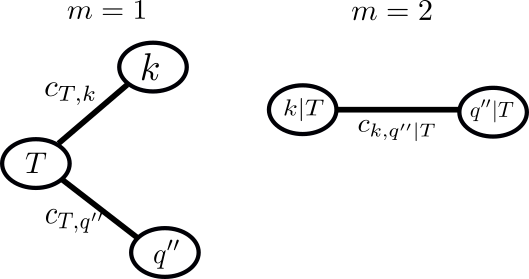
\includegraphics[width=0.4\linewidth]{figs/theory/c_vine_3var}
    \caption{C-vine on 3 variables: $\{T,q'',k\}$.}
    \label{fig:cvine3var}
\end{figure}

In this work it is assumed that the cladding surface temperature and near-wall TKE are uncorrelated with the boundary heat flux.  The justification is as follows.

Relative variations in boundary heat flux are very small over a CTF face $(\pm 5\%)$ provided that a CTF face represents a small (approximately $1 [cm^2]$) localized patch on the rod surface.  Large absolute heat fluxes of approximately $80 [W/cm^2]$ are possible on the cladding surface of fuel in a typical PWR.  However, high axial and azimuthal gradients of boundary heat flux on the rod surface are not typical under standard operating conditions.  High thermal gradients lead to thermal induced stresses on the cladding which can promote rod bowing or, extreme in conditions, fuel failure.
%Additionally, figures \ref{fig:crud_sensi1} to \ref{fig:crud_sensi3} show that the sensitivity of the crud growth rate to the boundary heat flux is small relative to the sensitivity of crud growth rates to surface temperature and local turbulent kinetic energy.

After applying the independence assumptions the original trivariate dependence model between the temperature, TKE, and boundary heat flux is reduced to a bivariate model in which the boundary heat flux is treated independently.  Applying the simplifying assumptions results in: $c_{T,q''}(u_T, u_{q''}) = 1$ and $c_{k,q''|T}(u_{k|T}, u_{q''|T}) = 1$. The simplified joint density is given by equation \ref{eq:simple_vine_model}:
\index{Copula!Vine Copula}
\begin{equation}
h(T, k, q'') \approx  f_T f_k, f_{q''} c_{T,k}(u_{T}, u_{k})  \cdot 1 \cdot 1
\label{eq:simple_vine_model}
\end{equation}
Where $u_T=F(T)$ and $u_k = F(k)$. $F(\cdot)$ denotes the CDF.
Following the independence assumption, the marginal density function of the outer cladding boundary heat flux is assumed to be a Dirac delta function centered on the value provided by CTF (VERA).  We will apply this assumption in all sections which follow.
Then in the $j^{th}$ CTF face the boundary heat flux marginal distribution is always given by equation \ref{eq:twall_dirac}.
\begin{equation}
f_{j,q''} = \delta_{(q''_{j, \mathrm{ctf}})}
\label{eq:twall_dirac}
\end{equation}


% ============ Copula Theory =============
\index{Copula}
%! TEX root = ../dissertation_gurecky.tex

%-----------------------------------------------------------------------------%
\subsection{Copula}

A copula is a function which relates marginal probability distributions to a multidimensional joint distribution.  Copula provide a flexible alternative to multidimensional Gaussian based models.  Copula are utilized in this work because of their ability to capture non-Gaussian dependence structure between two or more correlated random variables, for instance temperature and the TKE at a given point on a rod's surface.  Furthermore, Sklar's theorem is used in this work in order to decompose joint distributions into a product of uni-variate marginal distributions and a copula function.  In this section, Sklar's theorem is provided along with examples of copula functions
and techniques to draw samples from them. 

The product rule of probability is shown in equation \ref{eq:prod_prob}.  To clarify notation used in this section: The comma denotes the conjunction ``and'' and the bar, $|$, is read ``given''.
\begin{equation}
P(x, y) = P(x) P(y | x)
\label{eq:prod_prob}
\end{equation}

The marginal distribution of a bivariate joint distribution $f(x, y)$ is given by equation \ref{eq:marg}.  The marginalization process is analogous to projecting the entire joint density onto a single axis.
\begin{equation}
f(x) = \int f(y) f(x|y) dy
\label{eq:marg}
\end{equation}

The cumulative density function, $F$ is defined as:
\begin{align*} 
F &= \mathbf{P}[X < x] = \int_{-\infty}^x f(x)dx \\
\end{align*}

A joint $d$ dimensional cumulative distribution is given by equation \ref{eq:joint_cdf}.
\begin{equation}
H(x_1, ... x_d) = \mathbf P[X_1 \leq x_1, ... X_d \leq x_d]
\label{eq:joint_cdf}
\end{equation}
Where $X_1, ... X_d$ are random variables.

The process of decomposing a multivariate distribution into uni-variate marginal
distributions and an object which describes their conditional dependence was
formalized by Sklar \cite{Sklar1959}.  Shown in equation \ref{eq:sklar1},  Sklar's Theorem
defines a \emph{copula} cumulative density function, $C$.
\index{Sklar's Thorem}

\begin{equation}
C(F_1(x_1), ... F_d(x_d)) = H(x_1, ... x_d)
\label{eq:sklar1}
\end{equation}
If $F_1, .. F_d$ are continuous, then $C$ is unique.  Conversely, if $C$ is a copula and $F_1, .. F_d$ are smooth cumulative destiny functions then the function $H$ is a joint cumulative distribution with margins $F_1, ... F_d$.  A proof is provided in Nelsen's introductory copula text \cite{Nelsen2006}.

Sklar also showed that the joint probability distribution, $h(x_1, ... x_d)$, can be computed from
constituent marginalized univariate distributions and the copula density, $c$.
\begin{equation}
h(x_1,\dots x_d)= c(F_1(x_1),\dots F_d(x_d))\cdot f_1(x_1)\cdot\dots\cdot f_d(x_d)
\label{eq:sklar2}
\end{equation}

For brevity, let $u_1, .. u_d$ represent samples from their CDFs as follows:
\begin{align*} u_1 &= F_1(x_1) \\ u_d &= F_d(x_d) \\ u &\in
[0, 1]
\end{align*}

Where the joint density of the copula, $c$, is given by equation \ref{eq:cop_pdf}:
\begin{equation}
c(u_1, ... u_d) = \frac{\partial C(u_1, ... u_d)}{\partial u_1 ... \partial u_d}
\label{eq:cop_pdf}
\end{equation}

Sklar's theorem enables one to construct
models for the margins separately from a model of the dependence structure.
When combined, the margins and the copula 
specify a multivariate probability density function.
Compared to rudimentary approaches based on covariance matrix dependence model,
a copula based approach can treat skewed dependence structures in which the
strength of dependence is allowed to vary depending on location in the parameter space.

\section*{Sampling Copula}
\label{sec:sampling_copula}

For simplicity, this section demonstrates how to draw correlated samples from bivariate copula.
Sampling from a bivariate copula is achieved by first defining a conditional distribution function and then applying the inverse probability integral transform.
Let $h$ represent the conditional distribution of $u_1$ given all other random variables $\{u_2, ... u_d\}$.  In the two dimensional case $h$ is given by equation \ref{eq:cop_h} \cite{Nelsen2006}:
\index{Copula!Sampling}

\begin{equation}
h(u_1 | u_2) = \frac{\partial C(u_1, u_2)}{\partial u_2}
\label{eq:cop_h}
\end{equation}

If the distribution $h$ is smooth and monotonic the inverse $h^{-1}$ exists.  For a bivariate Gaussian copula with a shape parameter $\theta_c=0.7$ the conditional distribution functions are shown in figures \ref{fig:gauss_h} and \ref{fig:gauss_hinv} for several values of the conditioning variable ($u_2$).  

\begin{figure}[!htbp]
	\centering
	\begin{minipage}{.45\textwidth}
		%
		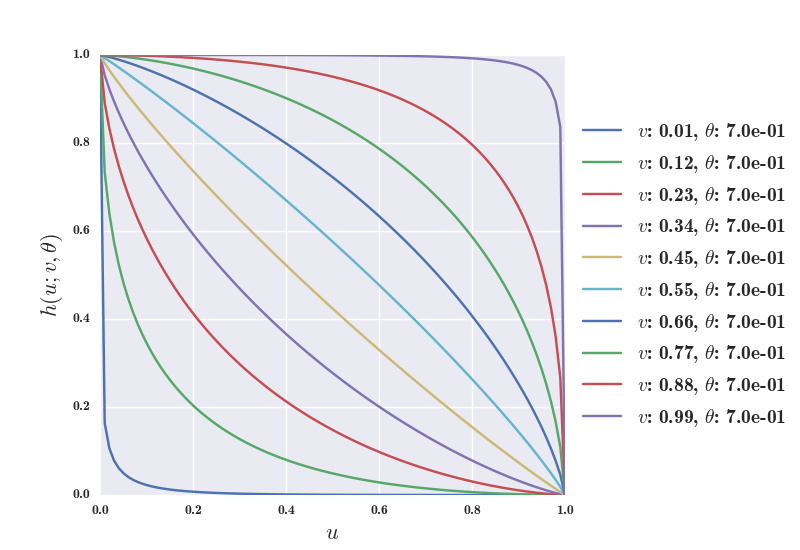
\includegraphics[width=7cm]{images/t_h_dist.png}
		\caption{The conditional $h$ \\ function vs. value of the \\ conditioning variable $u_2$ \\ for a Gaussian copula with $\theta_c=0.7$.}
		\label{fig:gauss_h}
	\end{minipage}%
	\begin{minipage}{.45\textwidth}
		%
		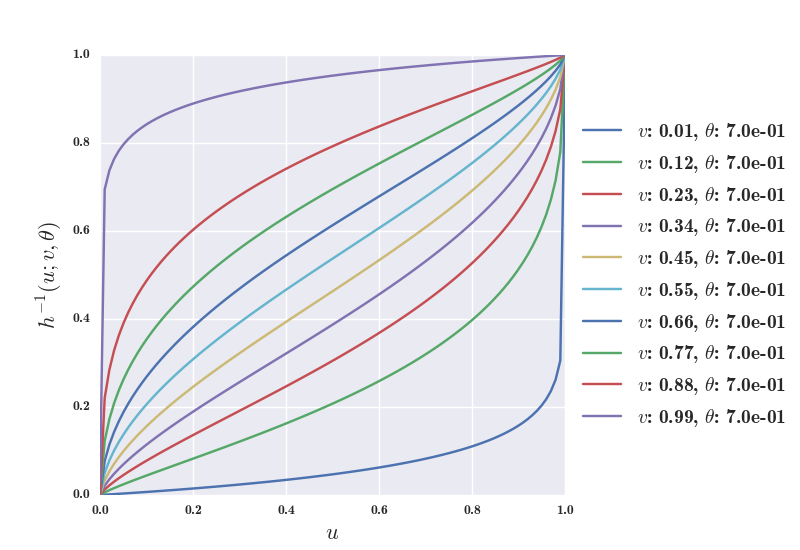
\includegraphics[width=7cm]{images/t_hinv_dist.png}
		\caption{$h^{-1}$ vs. value of the conditioning variable $u_2$ for a Gaussian copula with $\theta_c=0.7$.\\}
		\label{fig:gauss_hinv}
	\end{minipage}
\end{figure}

Computing the inverse analytically is oftentimes not possible for some classes of copula and therefore, the more general method shown in equation \ref{eq:h_inv_sample} is used.
A random vector of length $N$ is drawn from the uniform distribution $\in [0, 1]$:  $\{\mathbf U_2\}$.  For each sample, $u_{2_i}$ in $\{\mathbf U_2\}$ the 1-D line search problem given in equation \ref{eq:h_inv_sample} is solved.  This produces a sample vector of length $N$: $\{\mathbf U_1\}$.

\begin{equation}
u_{1_i} = \mathrm{argmin}_{u_1} \left[ h(u_1|u_{2_i}) - u_{2_i} \right],\ \mathrm{with}\ 0 < u_1 < 1
\label{eq:h_inv_sample}
\end{equation}

The resulting correlated sample vectors $\{\mathbf U_1, \mathbf U_2\} \in [0,1]^2$ are distributed according to the copula, $c$, and have uniform margins.  An example of random samples drawn from a Gaussian copula are shown in figure \ref{fig:gauss_samples}.  The smooth Gaussian copula PDF is provided in figure \ref{fig:gauss_pdf}.

\begin{figure}[!htbp]
	\centering
	\begin{minipage}{.45\textwidth}
		%
		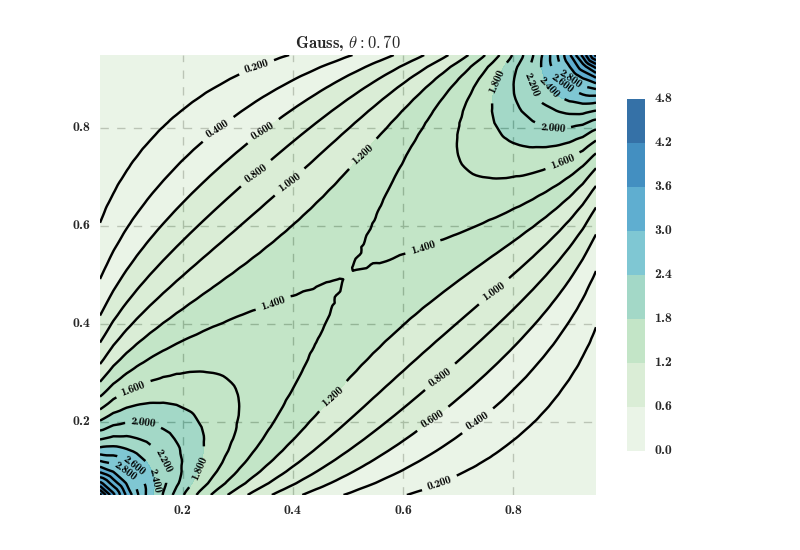
\includegraphics[width=9.2cm]{images/gauss_copula_pdf.png}
		\caption{Gaussian copula density\\ with $\theta_c=0.7$.}
		\label{fig:gauss_pdf}
	\end{minipage}%
	\begin{minipage}{.45\textwidth}
		%
		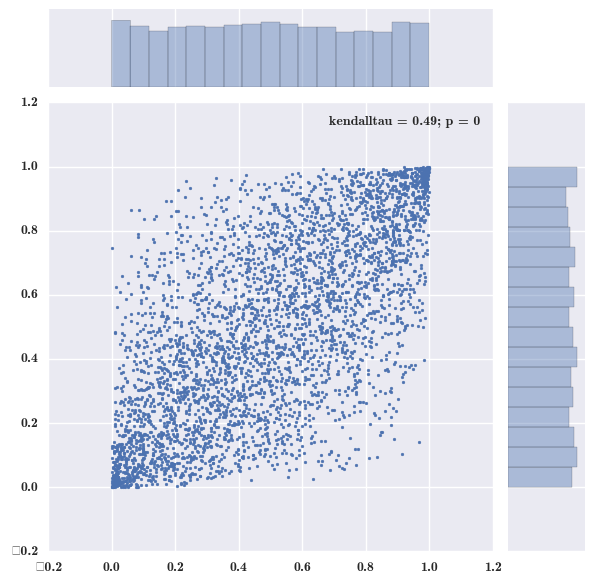
\includegraphics[width=7cm]{images/gauss_samples.png}
		\caption{Samples drawn from Gaussian copula\\ with $\theta_c=0.7$.}
		\label{fig:gauss_samples}
	\end{minipage}
\end{figure}

To apply arbitrary margins $F_1$ and $F_2$ we employ, again, the inverse probability transform. 
Correlated samples are then drawn according to:
\begin{eqnarray}
\mathbf X = & F_1^{-1}(\mathbf U_1) \\
\mathbf Y = & F_2^{-1}(\mathbf U_2)
\end{eqnarray}
The sample vectors $\{\mathbf X, \mathbf Y\}$ are distributed according to the joint density, $C(F_1, F_2)$.  An example bivariate sample set with exponentially distributed margins and a Gaussian copula is shown in figure \ref{fig:gauss_samples_scaled}.  In the example figure both margins follow an exponential distribution given by $f(x)=\lambda e^{-\lambda x}$ with $\lambda=2\mathrm{E-}3$.

\begin{figure}[!htbp]
	\centering
	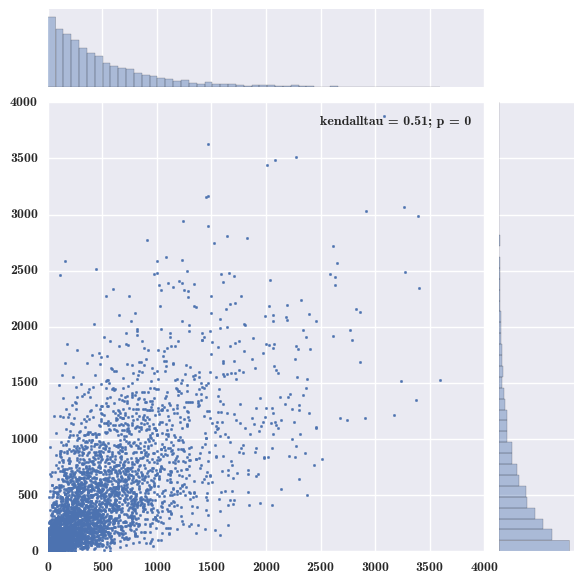
\includegraphics[width=9cm]{images/gauss_samples_scaled.png}
	\caption{Samples drawn from Gaussian copula with exponential margins.}
	\label{fig:gauss_samples_scaled}
\end{figure}


\section*{Copula Families}

A wide range of copula functions are available in the literature.  In order to satisfy the definition of a copula several criteria must be met:
\begin{enumerate}
	\item Must integrate to one on $[0, 1]^n$
	\item Must have uniform marginal distributions (as shown in figure \ref{fig:gauss_samples}).
	\item When one argument to the joint copula CDF is zero, the CFD is zero:
	\begin{equation}
	C(u_1, u_2, ... 0, ... u_d) = 0
	\end{equation}
	\item When one argument to the joint copula CDF is $u\in[0,1]$ and all other arguments are one, the CFD takes a value equal to $u$:
	\begin{equation}
	C(1, 1, ... u, ... 1) = u
	\end{equation}
\end{enumerate}

Examples of valid copula are given in figure \ref{fig:montage_cop}.  A wide range of skewed dependence structures can be represented by considering only a few copula families.  Each copula can be rotated to accommodate both positive or negative dependence.

\begin{figure}[!htbp]
	\centering
	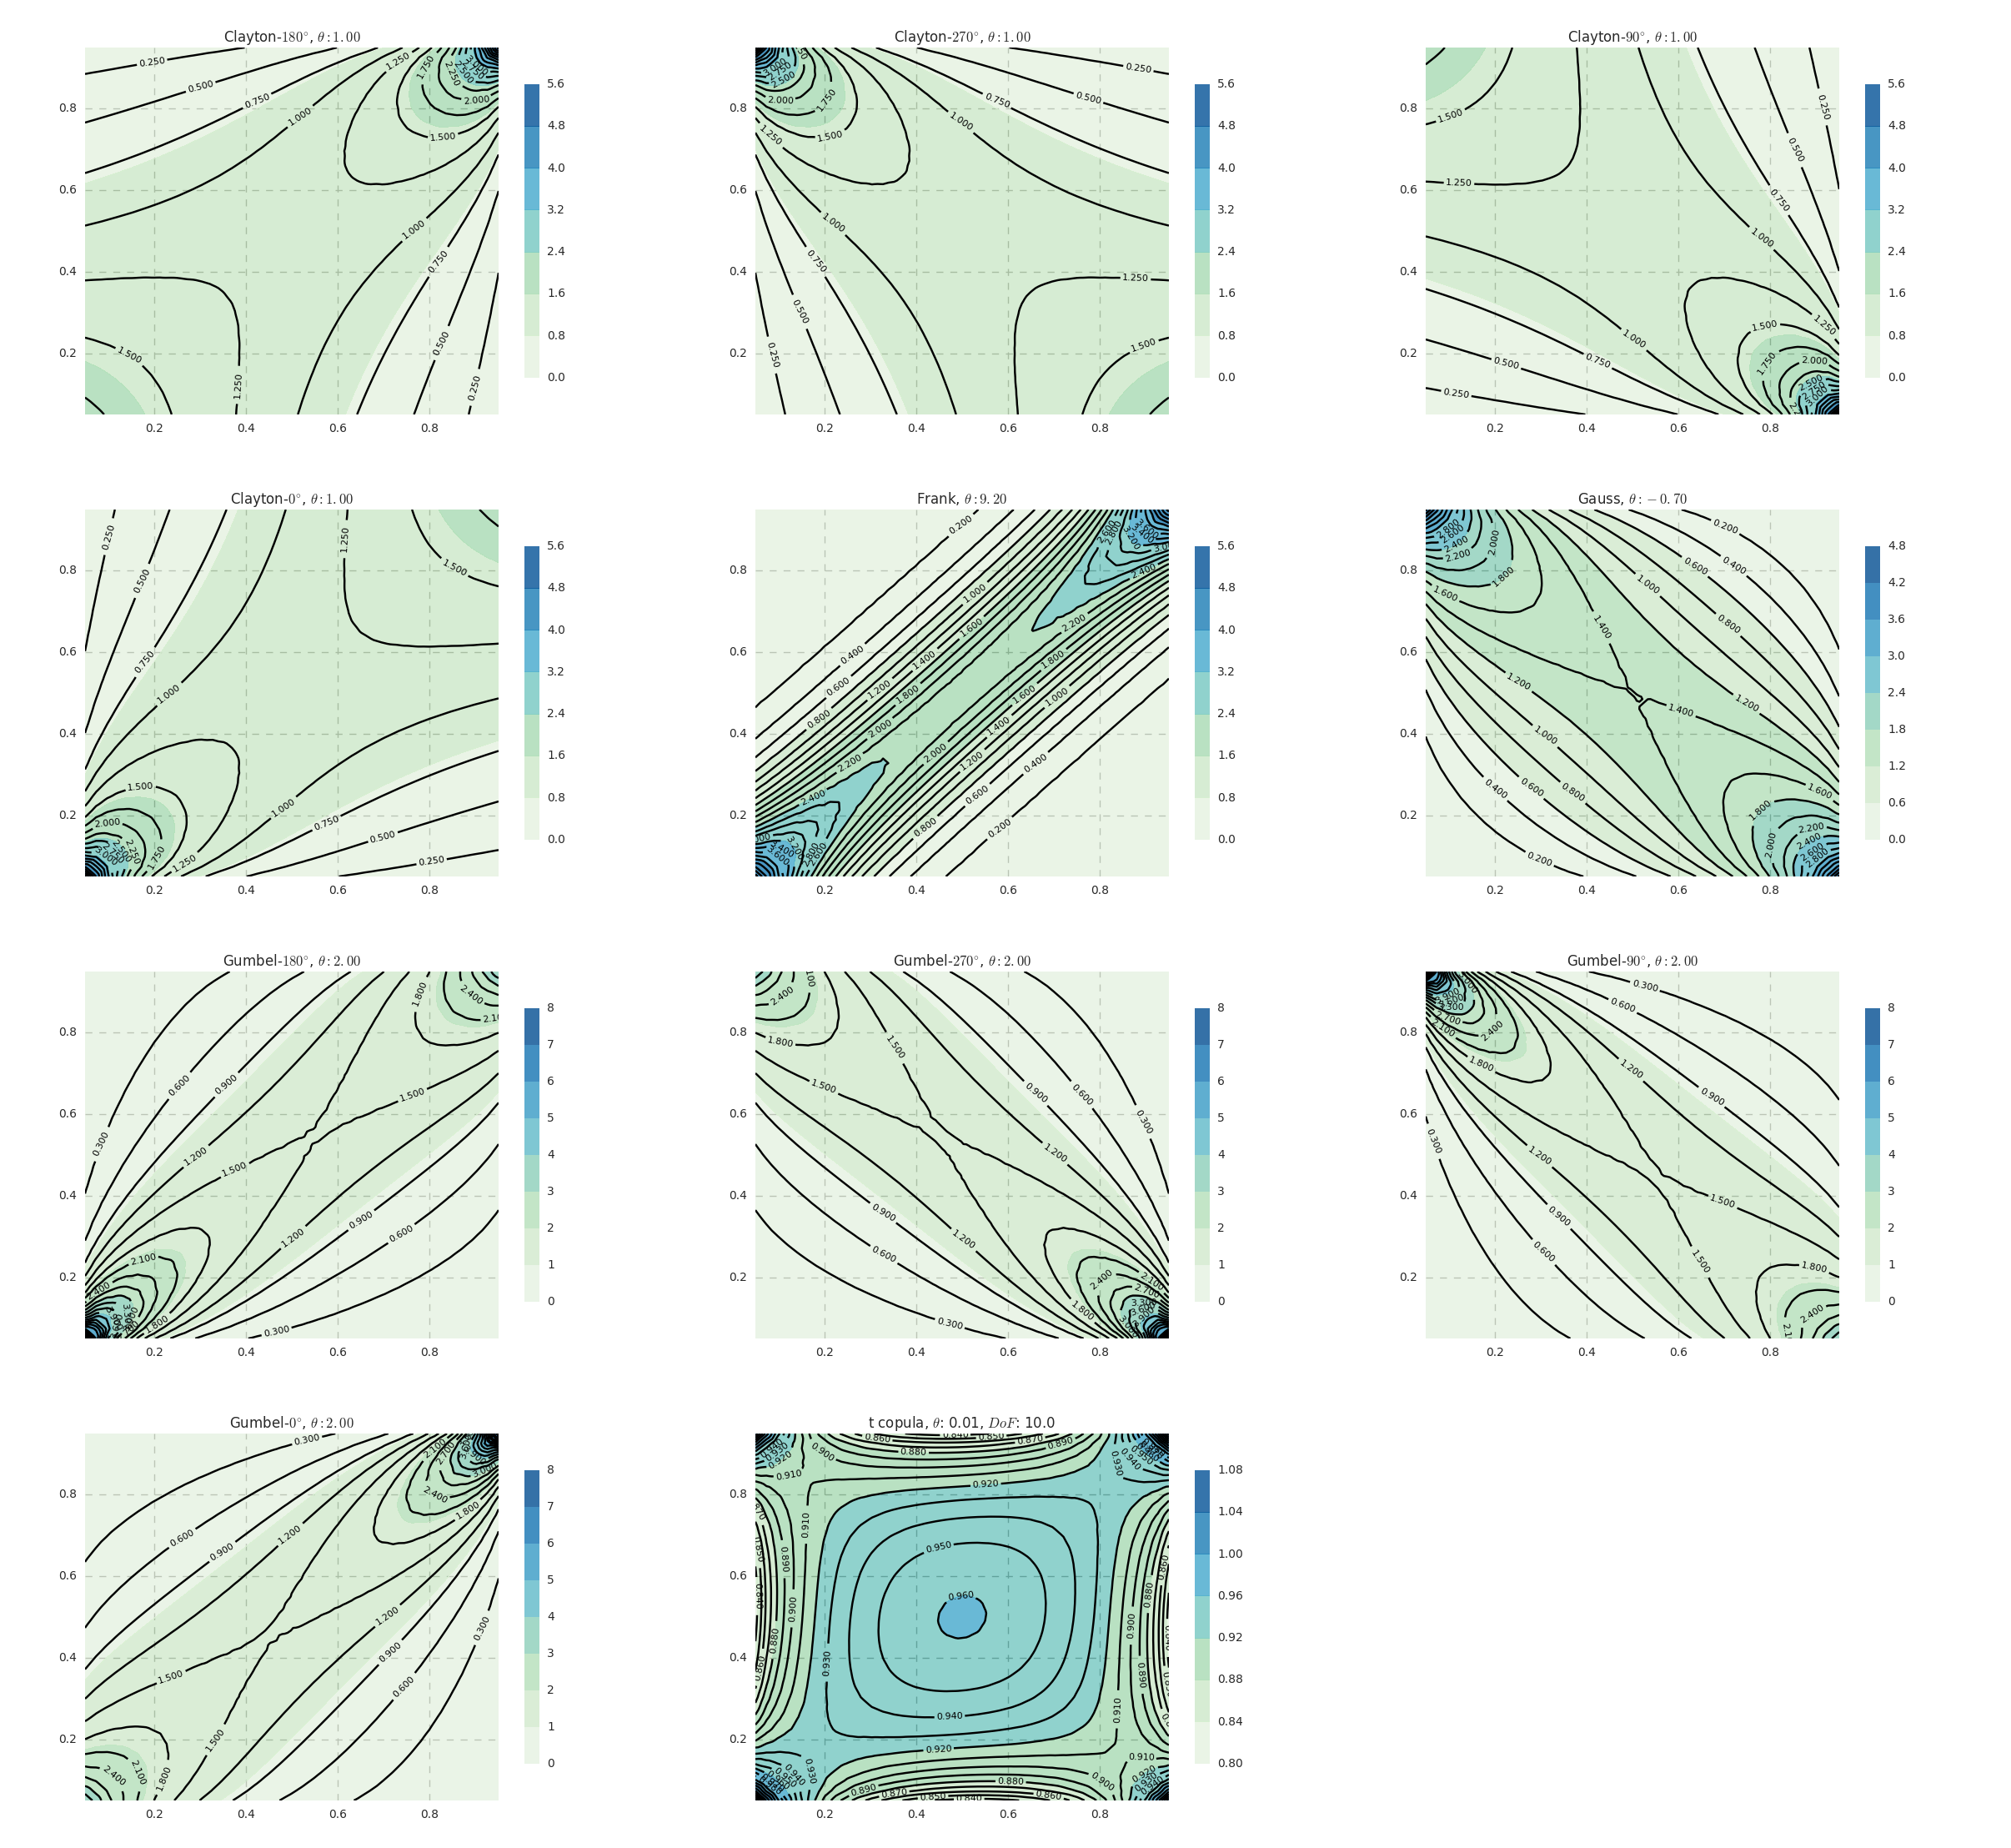
\includegraphics[width=18cm]{images/montage_copula_pdf.png}
	\caption{Examples of bivariate copula PDFs.}
	\label{fig:montage_cop}
\end{figure}

\subsection{Fitting Copula}
\label{sec:fitting_copula}

Fitting copula to empirical data can be carried out by the method of maximum likelihood (ML).  Consider the bivariate case where $N$ sample pairs, $\{w_i, v_i\}_{i\in [ 1,N ] }$  are known. The likelihood function for a copula is given by equation \ref{eq:lik}.  The likelihood is a function of the distribution parameter $\theta_c$ with the data, $\{\mathbf w,\mathbf v \}$, held fixed. When integrated over all possible parameter values the integrated result does not necessarily take on a value of unity and therefore cannot be strictly interpreted as a probability density. Each constituent factor in the likelihood function can be interpreted as the relative likelihood that the sample pair $\{w_i, v_i\}$ arose from the copula density function with parameter $\theta_c$.
\index{Copula!Fitting}

\begin{equation}
    \mathcal{L}(\theta_c;\mathbf w,\mathbf v)= \prod_{i=1}^N c(w_i, v_i|\theta_c)
\label{eq:lik}
\end{equation}

Where $\theta_c$ is the free copula shape parameter.
Typically the negative log-likelihood, $-\mathrm{ln}\mathcal{L}$, is used in when performing ML estimation of a distribution parameter since the problem is typically cast in terms of a minimization problem.  
\begin{equation}
\hat \theta_{c,ML} = \mathrm{argmin}_{\theta_c}[-\mathrm{ln}\mathcal{L}(\theta_{c} ; \mathbf w, \mathbf v)]
\label{eq:nlog_lik}
\end{equation}
\index{Maximum Likelihood}

To minimize the negative log likelihood in equation \ref{eq:nlog_lik}  one computes the partial derivative with respect to $\theta_c$ and finds the value $\hat \theta_{c,ML}$ for which this expression reaches zero.  This can be carried out by Newton's method.  If the partial derivatives of the copula's negative log likelihood are impossible to compute analytically one can estimate them by finite difference.

In order to determine which copula family best represents the data, an arsenal of statistical tests can be applied to select the copula which best fits the data.  Here, we consider two methods:  (1) Comparing Akaike information criterion (AIC) and (2) graphically comparing each fitted copula.  

The AIC is computed by equation \ref{eq:cop_aic}.
\begin{equation}
\mathrm{AIC} = 2k - 2\mathrm{ln}(\mathcal{L})
\label{eq:cop_aic}
\end{equation}
Where $k$ is the number of free parameters in the model.  The AIC penalizes models with larger numbers of parameters. 
Automated copula selection is achieved by selecting the copula that obtains the lowest AIC score.

A graphical method of copula selection was proposed by Barbe et. al. (1996) \cite{Barbe1996}.  In this method each trial copula's Kendall's function, $K_c(t)$ is plotted against an empirical estimate of this function, $\hat K_c$.  Given $d$ random variables $\mathbf U=\{U_1, ... U_d\}$ distributed according to some $d$ dimensional copula, $C$, Kendall's function is given by \ref{eq:Kc} \cite{Joe2015}.
\begin{equation}
K_c(t; C) = \mathrm P \left[C(\mathbf U) \leq t; \mathbf{U} \sim\ C\right]
\label{eq:Kc}
\end{equation}

\begin{figure}[!htbp]
	\centering
	\begin{minipage}{.45\textwidth}
		%
		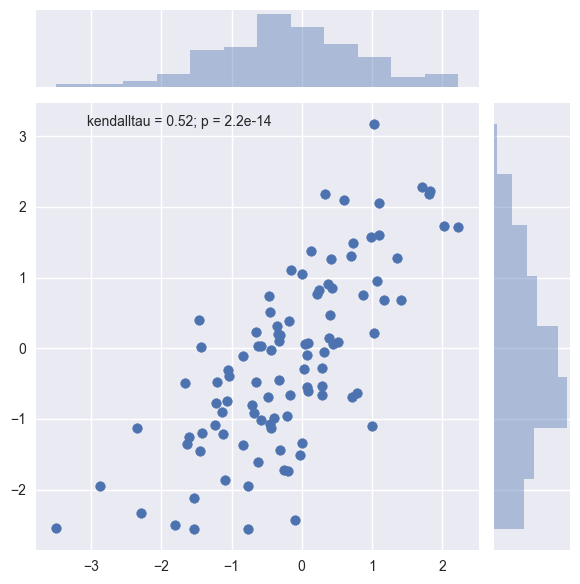
\includegraphics[width=6.5cm]{images/original_stocks.png}
		\caption{Ficticious bivariate \\ data set.}
		\label{fig:biv_data_ex}
	\end{minipage}%
	\begin{minipage}{.45\textwidth}
		%
		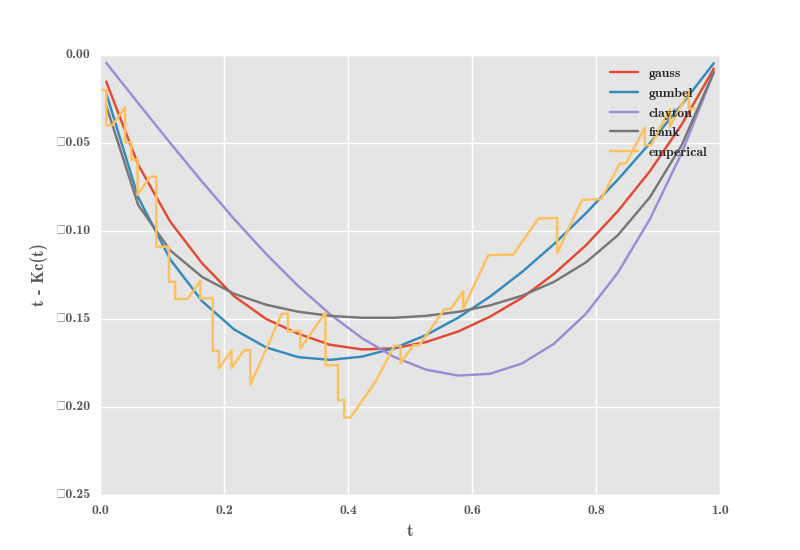
\includegraphics[width=9cm]{images/ktau_function_plot1.png}
		\caption{Graphical comparison of  \\ Kendall's distribution for \\ several fitted copula.}
		\label{fig:kc_fn_compare}
	\end{minipage}
\end{figure}
For example, by graphical inspection of figure \ref{fig:kc_fn_compare}, the Gumbel copula is the best fit to the original data set.  This visual process can be automated by computing and comparing $||\hat K_c(t) - K_c(t)||$ for each trial copula.

\subsection*{Kendall's Tau}

Kendall's tau is a measure of concordance.  Consider two correlated and uniformly distributed random variables, $X, Y$.
%  If a rank $x_{(i)}$ is drawn for the first variable, the likelihood that you will also have drawn the rank $y_{(i)}$ of the second to be at least as great as the first is proportional to Kendall's tau.  More precisely, 
Let $(X_1, Y_1)$ and $(X_2, Y_2)$ be identically distributed random vectors from some joint cumulative distribution so that individual samples from $X\ and\ Y$ will take on values in $[0,1]$, then Kendall's tau is given by equation \ref{eq:ktau} \cite{Nelsen2006}.  
\index{Kendall's Tau}

\begin{equation}
\rho_\tau = P[(X_1 - X_2)(Y_1-Y_2)>0] - P[(X_1 - X_2)(Y_1 - Y_2)<0]
\label{eq:ktau}
\end{equation}

In the case of Archimedean copula, $\rho_\tau$ is directly related to the copula's parameter, $\theta_c$.
Equation \ref{eq:tauar} relates an Archimedean copula's parameter to $\rho_\tau$.  This is useful since if one can estimate $\rho_\tau$ from the empirical data and the copula type is known, one can quickly compute the copula's shape parameter without resorting to the method of ML.

\begin{equation}
\rho_\tau = 1 + 4 \int_0^1 \frac{\varphi(\theta_c,t)}{\varphi'(\theta_c, t)}dt
\label{eq:tauar}
\end{equation}
Where $\varphi(t)$ is the copula's generator function and $\varphi'(t)$ is the first derivative of the generator function with respect to $t$. A list of copula generator functions may be found in introductory copula texts \cite{Nelsen2006}.

%\subsection*{Archimedean Copula}

%Archimedean copula are defined by the relationship.

%Where $\psi$ is a monotonically decreasing and convex function.

%A simplification can be made when fitting Archimedean copula since there is a one-to-one relationshipt between $\rho_\tau$ and the copula's shape parameter, $\theta_c$.




\subsection{Sample Quantiles}
\label{chap:quantiles}

Here a non parametric representation of univariate distributions is given by utilizing a set of sample quantiles.
Let the quantile function be represented by $Q=F^{-1}$ where $F$ is a cumulative density function (CDF).
\index{Cumulative density function}

%\begin{figure}[H]
%    \centering
%    \includegraphics[width=0.3\linewidth]{../proposal/slides/seminar_slides/figs/margins_cdf_2}
%    \caption[CDF from quantiles.]{Piecewise linear CDF interpolated from a set of quantiles.}
%    \label{fig:marginscdf2}
%\end{figure}

\index{Quantiles}
The $\tau^{th}$ quantile is $q_\tau = Q(\tau); $ where $\ F(t)=P[T \leq t]$.
$\tau \in [0, 1]$. The quantile loss function is given by equation \ref{eq:qloss_fn} and depicted in figure \ref{fig:qloss}.
\begin{equation}
\mathcal W_\tau( u) =  u \cdot (\tau - \mathbb{I}_{( u < 0)})
\label{eq:qloss_fn}
\end{equation}
Where $\mathbb{I}$ is the indicator function which returns 1 if the argument is true and 0 otherwise.
In order to estimate a sample quantile, $\hat q_\tau$, given the empirical CDF $F$, minimize: $\E[\mathcal W_\tau(T - q_\tau)]$ where $T$, the temperature, is treated as a random variable distributed according to $F_T$.  Considering a sample set $\{T_0, T_i, \dots T_N \}$ the desired quantile $q_\tau$ may be estimated by equation \ref{eq:qtau_est}.
\begin{equation}
            \left.\begin{aligned}
            \hat q_{\tau} &= argmin_{q_\tau} \E[\mathcal W_\tau(u)];\ \  u = T - q_\tau  \\
            \approx & argmin_{q_\tau}  \frac{1}{N} \sum_i^N \mathcal W_\tau(u_i); \ u_i = T_i - q_\tau \\
            \approx & argmin_{q_\tau} \left[ (1-\tau) \sum_{T \leq q_\tau}( T_i - q_\tau ) - \tau \sum_{T > q_\tau} (T_i - q_\tau) \right]
            \end{aligned}\right.
            \label{eq:qtau_est}
\end{equation}
\index{Quantiles!Loss Function}

%\begin{figure}[H]
%    \centering
%    \includegraphics[width=0.4\linewidth]{../proposal/slides/seminar_slides/figs/q_loss}
%    \caption[Quantile loss function.]{Quantile loss function.}
%    \label{fig:qloss}
%\end{figure}

\begin{figure}[H]
	\centering
	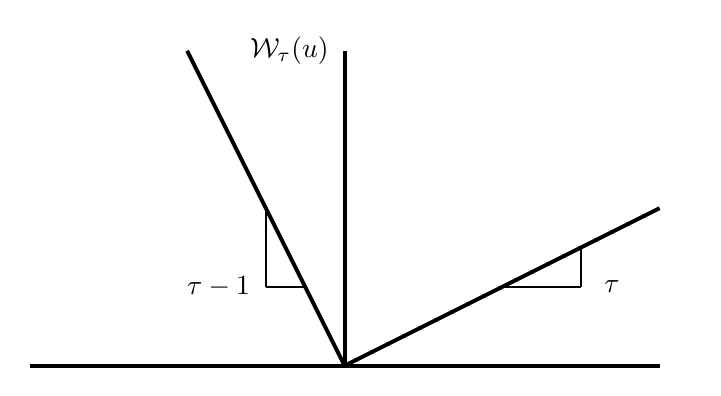
\begin{tikzpicture}
	% scalingn params
	\pgfmathparse{2.0}\let\s=\pgfmathresult
	% x y axes
	\draw [line width=0.05cm] (-2.0*\s, 0) -- (2.0*\s, 0);
	\draw [line width=0.05cm] (0.0, 0.0) -- (0.0, 2.0*\s);
	% Plot lines
	\draw [line width=0.05cm] (0.0, 0.0) -- (-1.0*\s, 2.0*\s);
	\draw [line width=0.05cm] (0.0, 0.0) -- (2.0*\s, 1.0*\s);
	% slope indicators
	\draw [line width=0.03cm]  (-0.5*\s, 0.5*\s) -- (-0.5*\s, 1.0*\s);
	\draw [line width=0.03cm]  (-0.5*\s, 0.5*\s) -- (-0.25*\s, 0.5*\s);
	%
	\draw [line width=0.03cm]  (1.5*\s,  0.5*\s)  -- (1.5*\s, 0.75*\s);
	\draw [line width=0.03cm]  (1.5*\s,  0.5*\s)  -- (1.0*\s, 0.5*\s);
	% figure text
	\node[text width=2cm] at (-0.1*\s,2.0*\s) {$\mathcal W_{\tau}(u)$};
	\node[text width=2cm] at (-0.5*\s,0.5*\s) {$\tau-1$};
	\node[text width=1cm] at (1.9*\s,0.5*\s) {$\tau$};
	\end{tikzpicture}
    \caption[Quantile loss function.]{Quantile loss function.}
\label{fig:qloss}
\end{figure}

In this work, a set of sample quantiles, $\hat \theta_\tau = \{\hat q_{\tau_0}, \dots, \hat q_{\tau_i}, \dots \hat q_{N_Q} \}$, are used to construct step-wise cumulative distributions, $\hat F$, for the cladding outer temperature and near-wall TKE surface fields.  $N_Q$ denotes the number of quantiles used in the CDF reconstruction and is a user set parameter. The stepwise quantile function with prescribed quantiles is given by equation \ref{eq:cdf_from_qtau} and depicted in figure \ref{fig:marginscdf2}.
\index{Quantiles!Emperical}

\begin{equation}
\hat F_{T}= Q^{-1}(T; \{\hat{\theta}_{\tau} \})
\label{eq:cdf_from_qtau}
\end{equation}
The reconstructed CDF can then in turn be used to build a histogram.  In place of the stepwise representation, a monotone piecewise cubic hermite interpolating polynomial (PCHIP) may be fit to the stepwise conditional quantile distribution to generate a differentiable CDF.
The PCHIP interpolation preserves monotonicity of the CDF if the provided quantiles are strictly monotone \cite{Fritsch80}.  This condition is enforced in the software; any violation of the monotone restriction would indicate a software bug in the quantile regression code.  Inverse transform sampling is used to draw samples from the univariate distributions.

\begin{figure}
	\centering
	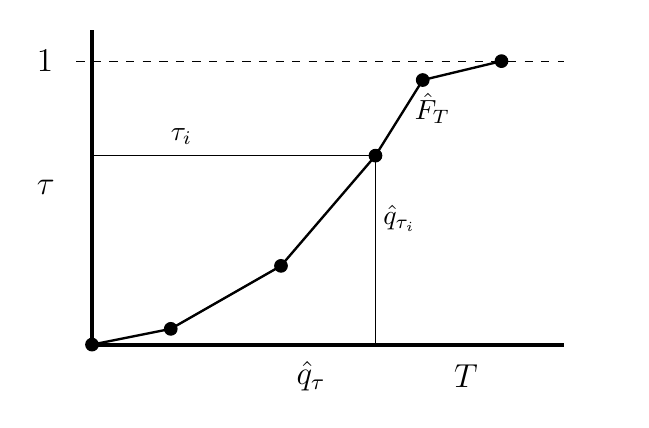
\begin{tikzpicture}
	% scalingn params
	\pgfmathparse{2.0}\let\s=\pgfmathresult
	% x y axes
	\draw [line width=0.05cm] (0, 0) -- (3.0*\s, 0);
	\draw [line width=0.05cm] (0.0, 0.0) -- (0.0, 2.0*\s);
	\draw [dashed]  (-0.1*\s, 1.8*\s) -- (3.0*\s, 1.8*\s);
	% plot nodes
	\draw [fill=black] (0.0, 0.0) circle (0.08cm);
	\draw [fill=black] (0.5*\s, 0.1*\s) circle (0.08cm);
	\draw [fill=black] (1.2*\s, 0.5*\s) circle (0.08cm);
	\draw [fill=black] (1.8*\s, 1.2*\s) circle (0.08cm);
	\draw [fill=black] (2.1*\s, 1.68*\s) circle (0.08cm);
	\draw [fill=black] (2.6*\s, 1.8*\s) circle (0.08cm);
	% Plot lines connecting nodes
	\draw [line width=0.03cm] (0, 0) -- (0.5*\s, 0.1*\s);
	\draw [line width=0.03cm] (0.5*\s, 0.1*\s) -- (1.2*\s, 0.5*\s);
	\draw [line width=0.03cm] (1.2*\s, 0.5*\s) -- (1.8*\s, 1.2*\s);
	\draw [line width=0.03cm] (1.8*\s, 1.2*\s) -- (2.1*\s, 1.68*\s);
	\draw [line width=0.03cm]  (2.1*\s, 1.68*\s) -- (2.6*\s, 1.8*\s);
	% mark a single node
	\draw [line width=0.02cm] (1.8*\s, 0) -- (1.8*\s, 1.2*\s);
	\draw [line width=0.02cm] (0.0, 1.2*\s) -- (1.8*\s, 1.2*\s);
	% figure text
	\node[text width=1cm] at (1.5, 1.32*\s) {$\tau_i$};
	\node[text width=1cm] at (2.1*\s, 0.8*\s) {$\hat q_{\tau_i}$};
	\node[text width=1cm] at (2.3*\s, 1.5*\s) {$\hat F_T$};
	\node[text width=1cm] at (-0.1*\s,1.0*\s) {\large $\tau $};
	\node[text width=1cm] at (-0.1*\s,1.8*\s) {\large $1 $};
	\node[text width=2cm] at (1.8*\s, -0.2*\s) {\large $\hat q_{\tau}$};
	\node[text width=2cm] at (2.8*\s, -0.2*\s) {\large $T$};
	\end{tikzpicture}
	\caption[CDF from quantiles.]{Piecewise linear CDF interpolated from a set of quantiles.}
	\label{fig:marginscdf2}
\end{figure}

Other strategies to approximate univariate density functions from a set of sample statistics are abundant.  One alternative to quantile regression is to relate sample moments to the parameters of some parametric distribution.  In this procedure a set of moment conditions is defined for the target parametric model.  Then the method of moments (MoM) can be used to determine the parameters of the parametric model which best satisfy the moment conditions in the L2 norm sense.  The MoM is applicable when the number of defined moment conditions is greater than or equal to the number of free distribution parameters.

Alternatively, one may construct a non-parametric univariate density given some set of predictive features by utilizing a set of predicted distribution cumulants.  The estimated cumulants, produced by evaluating a trained machine learning model, may be used to build an Edgeworth series expansion \cite{hall1997}.  It remains as future work to determine if cumulants or traditional moments behave in a predictable manner as a function of local core conditions.

% If the sample moments or cumulants cannot be acurately predicted by a data driven machine learning model, or some physical model linking the sample moments of the temperature and TKE fields to local core conditons cannot be found, it becomes intractable to use either the MoM or Edgworth series expansion approach.   Furthermore, if there exists a high sensitivity to purtibations in the transfer function relating the sample moments to the distribution paramters.  In simple cases method of moments can be understood by studying the linear operator in equation ().  If this operator has a large condition number then small errors made in the prediction of the momments will corrospond to large errors in the prediction of the model distribution parameters.  For these reasons, it is left as future work to investigate these strategies for marginal distribution recovery from moments or cumulents.  Instead, this work employes a forward quantile regression strategy for which the uncertainties in the predicted quantiles can be quantified in a straight forward manner.

It can be shown that the sample quantiles are distributed according to equation \ref{eq:theory_qdist_1}.  This directly follows from the distribution of the order statistics \cite{mosteller1946}.  The theoretical distribution of the quantiles is Gaussian in the large sample limit.  The large sample behavior of the quantiles is demonstrated for a normal random variable in figure \ref{fig:normal_q_theory} and a beta random variable in figure \ref{fig:beta_g_theory}.  When benchmarking or validating quantile predictions it is essential to check that the predictions follow the expected Gaussian behavior.  For the quantile regression procedures employed in this work, this check is performed in section \ref{chap:GBRT}.  Deviance from the expected behavior would indicate additional model-induced quantile prediction variance or if skewness is observed, bias introduced by the quantile regression model.  In the current application it is important to estimate uncertainties inherent to the sample quantile estimation procedure so such uncertainties may be propagated into the crud integration procedures.
\index{Quantiles!Theoretical distribution}

\begin{align}
    q_p &\sim \mathcal N \left( F_T^{-1}(p), \sigma^2_{q_p} \right) \nonumber \\
    \sigma^2_{q_p} &= \frac{p(1 - p)}{n[f_T(F_T^{-1}(p))]^2}
    \label{eq:theory_qdist_1}
\end{align}

In equation \ref{eq:theory_qdist_1} the variance associated with a sample quantile depends on the CDF and PDF of the true distribution function of interest.  The underlying CDF from which a sample population is typically unknown and the goal is often to infer properties of this distribution from the sample population.  Therefore, it is not possible to employ equation \ref{eq:theory_qdist_1} directly to compute the variance of a given sample quantile unless the underlying CDF is known.  Note that this is indeed the case in section \ref{chap:GBRT} where the large sample quantile theory is employed to check the residuals of a quantile regression procedure because the underlying distribution of the data was prespecified to be Gaussian.  However, from more complex cases where the nature of the distribution functions is unknown, such as with raw CFD data, equation  \ref{eq:theory_qdist_1} is not directly useful but still can be used to aid interpretation of the quantile regression predictions.

\begin{figure}[H]%
    \captionsetup[subfigure]{justification=centering}
    \centering
        \subfloat[][Empirical quantiles for a normal distribution. \\ 500 trials shown. $0.1, 0.5, 0.9$ quantiles \\ denoted by dashed verticle lines.]{{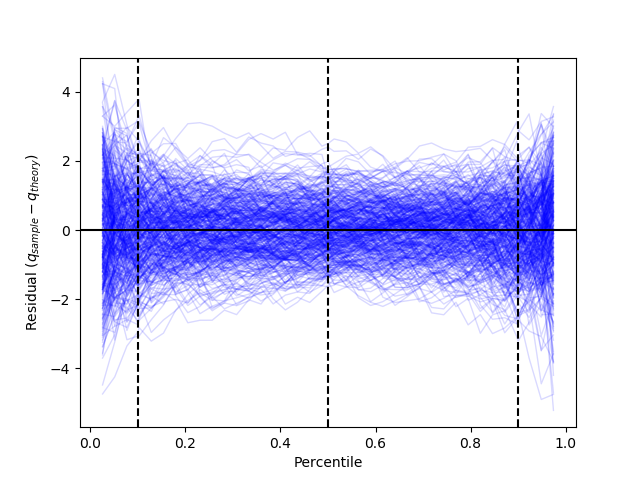
\includegraphics[width=0.52\linewidth]{figs/quantile_theory/q_gauss_residual} }}\hspace*{-1.0em}%
        \subfloat[][Empirical vs theoretical $0.1$ quantile \\ distribution.]{{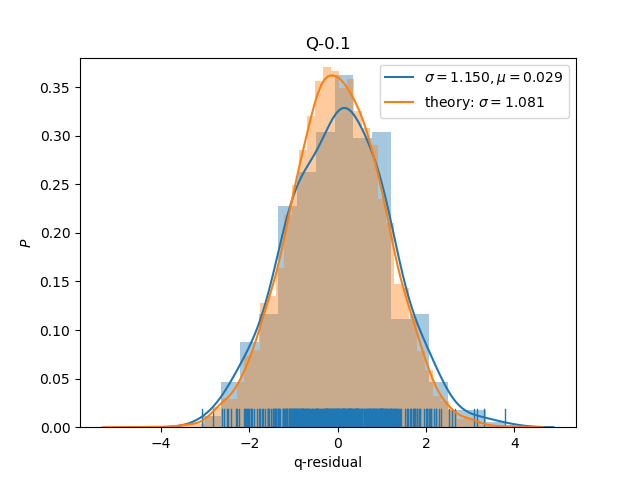
\includegraphics[width=0.52\linewidth]{figs/quantile_theory/q_gauss_residual_conditional_0_1} }}\hspace*{-1.0em}%
        \\
        \subfloat[][Empirical vs theoretical $0.5$ quantile \\ distribution.]{{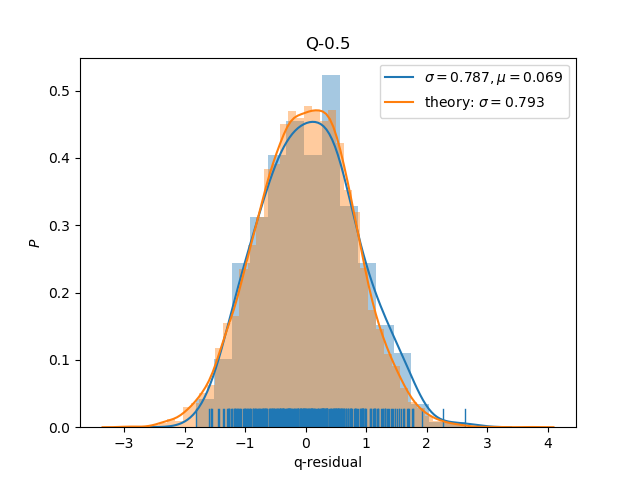
\includegraphics[width=0.52\linewidth]{figs/quantile_theory/q_gauss_residual_conditional_0_5} }}\hspace*{-1.0em}%
        \subfloat[][Empirical vs theoretical $0.9$ quantile distribution.]{{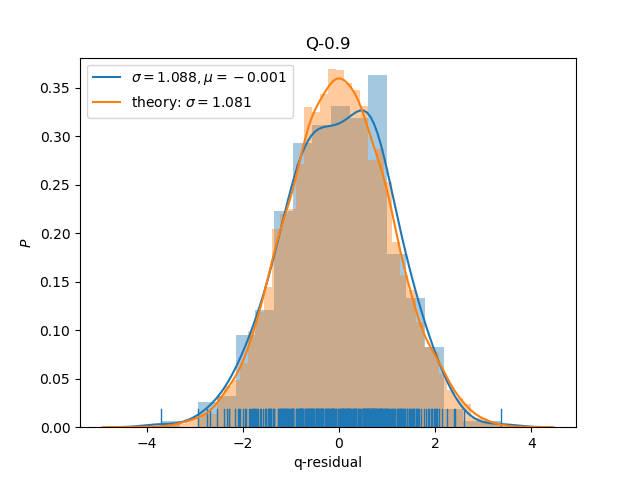
\includegraphics[width=0.52\linewidth]{figs/quantile_theory/q_gauss_residual_conditional_0_9} }}%
    \qquad
    \caption[Distribution of quantiles for a normally distributed RV.]{Distribution of quantiles for a normally distributed RV: $X \sim \mathcal{N}(0, 10)$.  Theoretical quantile standard deviation given by equation \ref{eq:theory_qdist_1}.}%
    \label{fig:normal_q_theory}%
\end{figure}

\begin{figure}[H]%\\
     \captionsetup[subfigure]{justification=centering}
    \centering
    \subfloat[][Empirical quantiles for a beta distribution. \\ 500 trials shown. $0.1, 0.5, 0.9$ quantiles \\ denoted by dashed verticle lines.]{{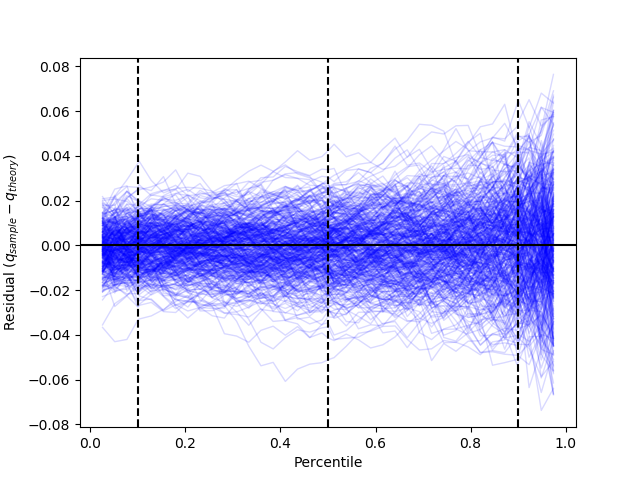
\includegraphics[width=0.52\linewidth]{figs/quantile_theory/q_beta_residual} }}\hspace*{-1.0em}%
    \subfloat[][Empirical vs theoretical $0.1$ quantile \\ distribution.]{{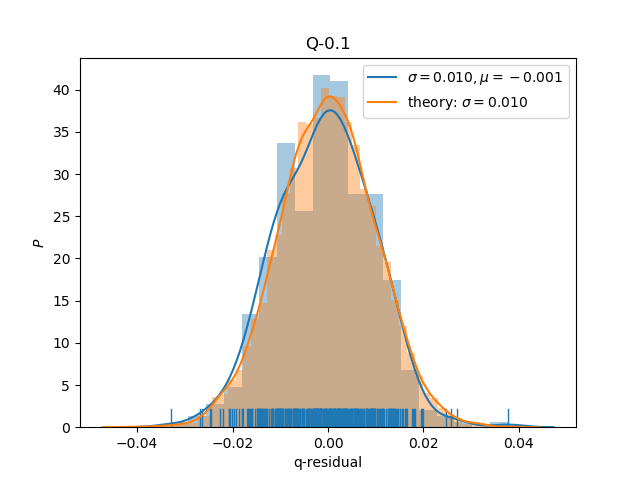
\includegraphics[width=0.52\linewidth]{figs/quantile_theory/q_beta_residual_conditional_0_1} }}\hspace*{-1.0em}%
    \\
    \subfloat[][Empirical vs theoretical $0.5$ quantile \\ distribution.]{{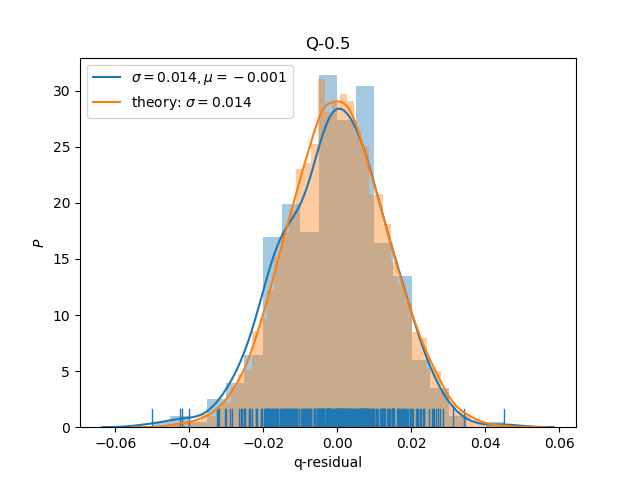
\includegraphics[width=0.52\linewidth]{figs/quantile_theory/q_beta_residual_conditional_0_5} }}\hspace*{-1.0em}%
    \subfloat[][Empirical vs theoretical $0.9$ quantile \\ distribution.]{{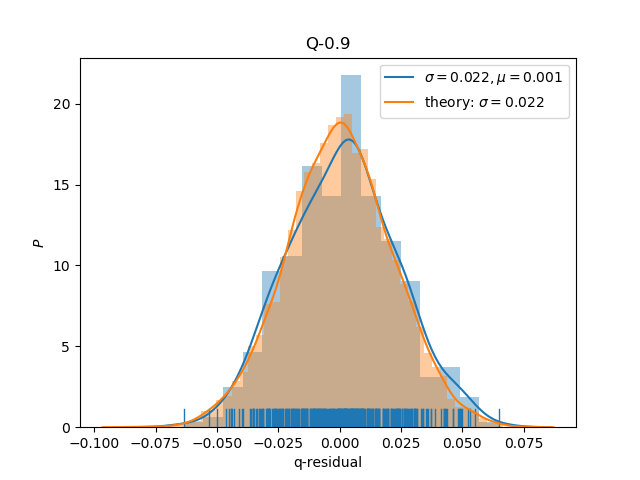
\includegraphics[width=0.52\linewidth]{figs/quantile_theory/q_beta_residual_conditional_0_9} }}%
    \qquad
    \caption[Distribution of quantiles for a beta distributed RV.]{Distribution of quantiles for a beta distributed RV: $X \sim \beta(2, 5)$}%
    \label{fig:beta_g_theory}%
\end{figure}

The sampled temperatures may be tallied over each CTF face to estimate the fractional area that exceeds some threshold temperature.  The probability of exceeding a threshold temperature is shown in equation \ref{eq:pr_thresh}.

    \begin{equation}
    p_e = Pr(T > T^*) = 1 - \int_0^{T^*} f_T dT
    \label{eq:pr_thresh}
    \end{equation}

    Let $q_p = F_T^{-1}(1 - p_e)$
    denote the quantile associated with the threshold probability, $p_e$.
    $F_T^{-1}$ is the inverse CDF function and $f_T$ is the probability density function of temperature on the patch.

    The sample quantile corresponding to $p_e$ is distributed according to:

   \begin{eqnarray}
    q_p &\sim \mathcal N \left( F_T^{-1}(p), \sigma^2_{q_p} \right) \\
    \sigma^2_{q_p} &= \frac{p(1 - p)}{n[f_T(F_T^{-1}(p))]^2}
    \end{eqnarray}

    The variance of upper tail probability mass estimate can be found by standard propagation of uncertainty principles:
   \begin{equation}
    \sigma_p^2 = \left(\frac{\partial p_e}{\partial q_p} \right)^2 \cdot \sigma_{q_p}^2 +\  HOT.
    \label{eq:pr_thresh_uncert}
    \end{equation}

    Where
   \begin{eqnarray}
    \frac{\partial p_e}{\partial q_p} &= \frac{\partial}{\partial q_p} \left( 1 - \int_0^{q_p} f_T dT \right) \nonumber \\
    &= \frac{\partial}{\partial q_p} \left( -F_T(q_p) + F_T(0) \right) \nonumber \\
    &= -f_T(q_p)
    \end{eqnarray}
    This dictates that estimates of extreme upper tail integrals carry large relative uncertainties.

%    The approximate large sample distribution for $p_e$ can be obtained by a change of variables, since $p_e$ and $q_p$ are related by:
%    \begin{equation}
 %   q_p = F_T^{-1}(1 - p_e)
%    \end{equation}
%    Where $F_T^{-1}$ is the inverse CDF.  $p_e$ is distributed according to:
%    \begin{equation}
%    f_{p_e} = f_{q_p} \left( F_T^{-1}(1-p_e), \sigma_{q_p}(p_e) \right) \cdot \left|{ \frac{\partial}{\partial p_e} F^{-1}(1-p_e) } \right|
%    \end{equation}


\subsection{Gradient Boosted Regression Trees}
\label{chap:GBRT}

A data driven machine learning model is used to predict quantiles, $\{ \hat \theta_\tau \}$, required to reconstruct cumulative density functions as shown in equation \ref{eq:cdf_from_qtau}.  The desired quantiles of the cladding surface temperature and TKE fields are conditioned upon the local core state denoted here by $\mathbf p$.  The vector $\mathbf p$ contains the local thermal hydraulic conditions in the core and local geometric grid and pin factors.  The purpose of this vector is to uniquely identify each CTF face in the core though some set of explanatory features.  The problem is then of conditional quantile prediction and this is performed by gradient boosted regression trees in this work.

\begin{figure}[H]
    \centering
    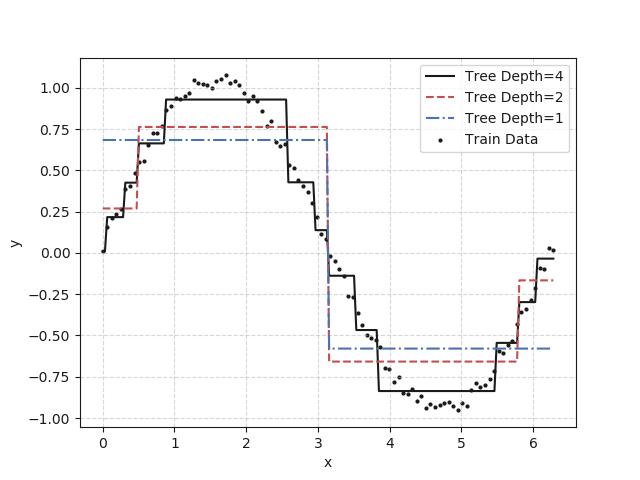
\includegraphics[width=0.59\linewidth]{../proposal/slides/seminar_slides/figs/cart}
    \caption[Regression tree stump.]{Single CART regression tree stump comparing a fit of depth 1 and 2 to the function $y=sin(x) + \varepsilon,\ x\in[0,2\pi], \varepsilon \sim \mathcal N(0,0.001)$.}
    \label{fig:cart}
\end{figure}

The modern gradient boosting algorithm was developed by Friedman et. al. (1998) \cite{friedman1998}, \cite{friedman2001}.  The development of generalized boosting was significant because it re-envisioned previous boosting algorithms such as AdaBoost as special cases of gradient boosting with specific loss functions.  Gradient boosting is a numerical optimization procedure carried out in function space with the goal of finding a function $\mathcal F_M$ that maps the inputs $\mathbf p$ to $y$ where $\mathcal F_M$ is given by equation \ref{eq:boosting_problem}.
\index{Gradient Boosting}

\begin{equation}
\mathcal F_M = \text{argmin}_{\mathcal F} \E_{y, \mathbf p} (L(y, \mathcal F(\mathbf p)))
\label{eq:boosting_problem}
\end{equation}
Where $L(\cdot)$ is a differentiable loss function.  $\mathbf p$ are known as predictive features and $y$ is the response.  The paired set $\{\mathbf p, y \}$ is referred to as the training data set.  In the standard gradient boosting algorithm the functional form of $\mathcal F$ is chosen to be an additive model of the form \ref{eq:single_cart_model}:
\begin{equation}
\mathcal F_M(\mathbf p, \mathbf{\gamma}, \mathbf a; \mathbf b) = \sum_{m=0}^M \gamma_m h_m(\mathbf p, a_m; b_m)
\label{eq:single_cart_model}
\end{equation}
Where $M$ is the number of constituent sub-models and $\{\gamma_m, a_m\}$ are coefficients and free parameters requiring fitting in each sub-model.  $b_m$ represent sub-model hyperparameters that are fixed at user set values.
Rather than fitting all sub-models simultaneously,
gradient boosting greedily fits the sub-models to the gradient of the loss function in a stage wise fashion as shown in algorithm \ref{alg:boosting}.  The loop depicted in line number 8-10 performs the computation of the loss function gradient at each boosted iteration $m$ in the algorithm.  In the literature the vector of gradients is sometimes referred to as the pseudo residuals vector since if the loss function is taken to be the L2 loss, the gradient of the loss is proportional to the residual vector as shown in equation \ref{eq:l2_loss_pseudo_r}.

\begin{align}
    (y_i - \mathcal F_{m}(x_i)) & \propto \frac{\partial [(y_i - \hat y_i)^2]}{\partial \hat y_i} \nonumber \\
     & \propto \frac{\partial (y_i^2 + \hat y_i^2 - 2y_i \hat y_i)}{\partial \hat y_i} = 2 \hat y_i - 2 y_i
    \label{eq:l2_loss_pseudo_r}
\end{align}

Each sub-model, $h_m$, is referred to as a weak learner and is defined to be a typical classification or regression tree (CART) depending on the problem context.  Methods for fitting, pruning the decision trees and optimizing the numerical implementation of finding the best splits when fitting the tree to the pseudo-residuals are left to Friedman et. al. \cite{friedman2002}.  Provided CART trees are used for the weak learners, the free (sub-) model parameters $a_m$ take the form of split locations and regional constants which are fitted to produce a piecewise constant predictor.  In this case the user set hyperparameters, $b_m$, are taken to be the maximum tree depth allowed when fitting each weak learner to the pseudo-residuals.

Examples of single dimensional fitted CART trees with a depth of 1 and 2 are shown in figure \ref{fig:cart}.  As the depth of a tree is increased the decision tree prediction converges onto the data; however, a single decision tree of large depth is prone to over fitting the data.  Decision trees produce a piecewise constant prediction, and therefore since the final boosted model is a linear combination of decision tree models (weak learners), the fitted boosted model is piecewise constant.

\begin{algorithm}[H]
    \captionsetup{labelfont={sc,bf}, labelsep=newline}
    \caption{Gradient boosting algorithm \cite{friedman2002}.}
    \begin{algorithmic}[1]
    \STATE \textbf{Initialization}
    \STATE (1) Training set $\{(p_i, y_i)\}_{i=1}^n$.
    \STATE (2) Differentiable loss function $L(y, \mathcal F(p))$.
    \STATE (3) Number of iterations ${{M}}$.
    \STATE (4)   Initialize model with a constant value:
        $\mathcal F_0(p) = \underset{\gamma}{\arg\min} \sum_{i=1}^n L(y_i, \gamma).$

    \FOR {${{m}} = 1$ to ${{M}}$}
        \STATE Compute the pseudo-residuals:
        \FOR {$i=1,\ldots,n $}
            \STATE $r_{im} = -\frac{\partial L(y_i, \mathcal F_{m-1}(p_i))}{\partial \mathcal F_{m-1}(p_i)}$
        \ENDFOR

        \STATE Fit a weak learner $h_m(p; a_m)$ to pseudo-residuals, $r_{m}$: \\
            $\ \ \ h^* = \underset{a_m}{\operatorname{arg\,min}}(||h_m(p; a_m) - r_m||)$ \\
            $\ \ $ Training data set is $\{(p_i, r_{im})\}_{i=1}^n$ \;

        \STATE Compute multiplier $\gamma_m$ :
        $\gamma_m = \underset{\gamma}{\operatorname{arg\,min}} \sum_{i=1}^n L\left(y_i, \mathcal F_{m-1}(p_i) + \gamma h^*_m(p_i)\right)$\;
        \STATE Update the model:
        $\mathcal F_m(p) = \mathcal F_{m-1}(p) + \nu \gamma_m h^*_m(p).$

    \ENDFOR
    \STATE Output $\mathcal F_M(p).$
    \end{algorithmic}
\label{alg:boosting}
\end{algorithm}
\index{Gradient Boosting!Algorithm}

Where $\nu$ is a tunable constant in $(0, 1]$ called the learning rate.  A value of $\nu < 1$ reduces the contribution of each weak learner in the final model.  Reducing the learning rate increases resilience to over fitting but results in a proportional increase in the number of boosted iterations to achieve the same level of convergence of the boosted tree chain.  Smaller values for the learning rate result in performing smaller steps in function space so we are less likely to overshoot the optimal function. Provided boosting produces a stage-wise additive model, overshoots are problematic since the final model carries memory of previous iterations.  A typical learning rate is $\nu\leq 0.05$ but a balance between computation time and model prediction accuracy on a testing set should be considered when setting this value.

For gradient boosted quantile regression, the loss function given by equation \ref{eq:qloss_fn} is substituted into algorithm \ref{alg:boosting}.
\begin{equation}
L(y, \mathcal F(p);\tau) = \left[ (1-\tau) \sum_{y \leq \mathcal F(p)}( y_i - \mathcal F(p) ) \right] - \left[ \tau \sum_{y > \mathcal F(p)} (y_i - \mathcal F(p)) \right]
\end{equation}
Where $\tau$ is the user set quantile of interest. For instance, if the 95\% percentile is desired then $\tau=0.95$.

% boosting tree results
%! TEX root = ../outline.tex

% \subsection{Gradient Boosted Regression Trees}

\begin{figure}[H]%
    \centering
    \subfloat[$\tau = 0.5$.]{{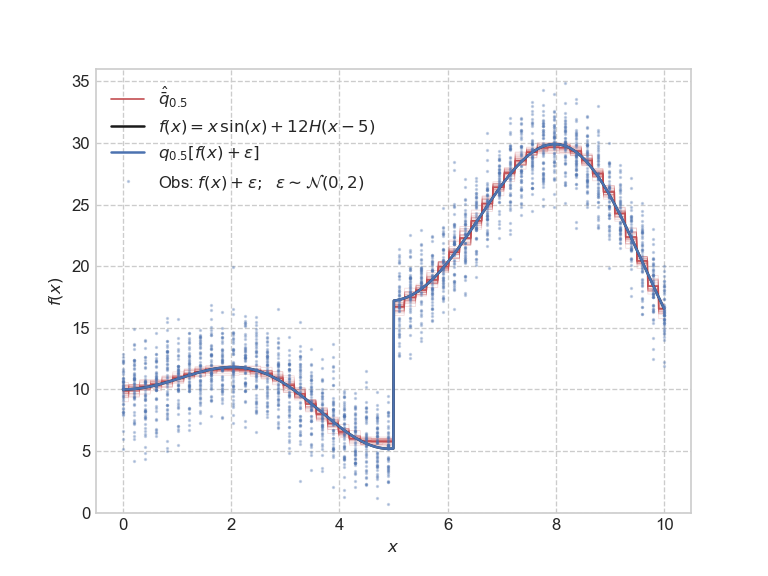
\includegraphics[width=0.53\linewidth]{figs/grad_boost/1d_boosted_regression_quantile_ex_0_5} }}\hspace*{-1.0em}%
    \subfloat[$\tau = 0.9$.]{{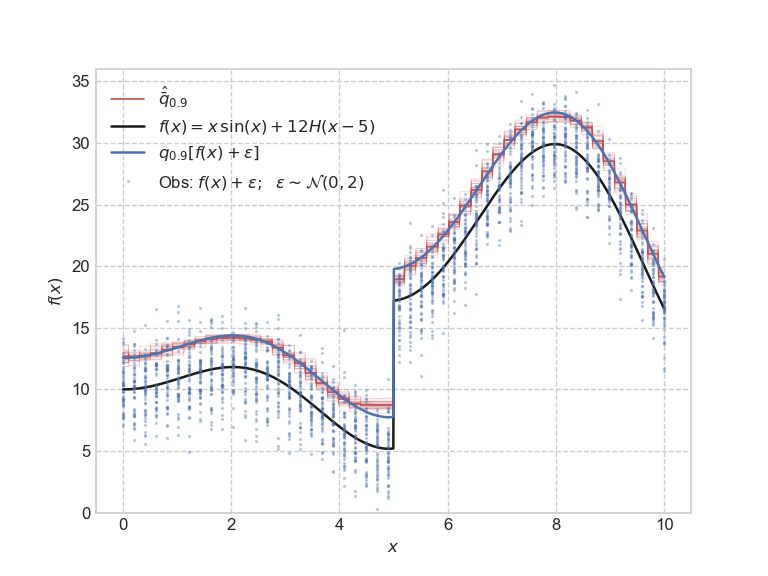
\includegraphics[width=0.53\linewidth]{figs/grad_boost/1d_boosted_regression_quantile_ex_0_9} }}\hspace*{-1.0em}%
    \\
    \subfloat[$\tau = 0.75$.]{{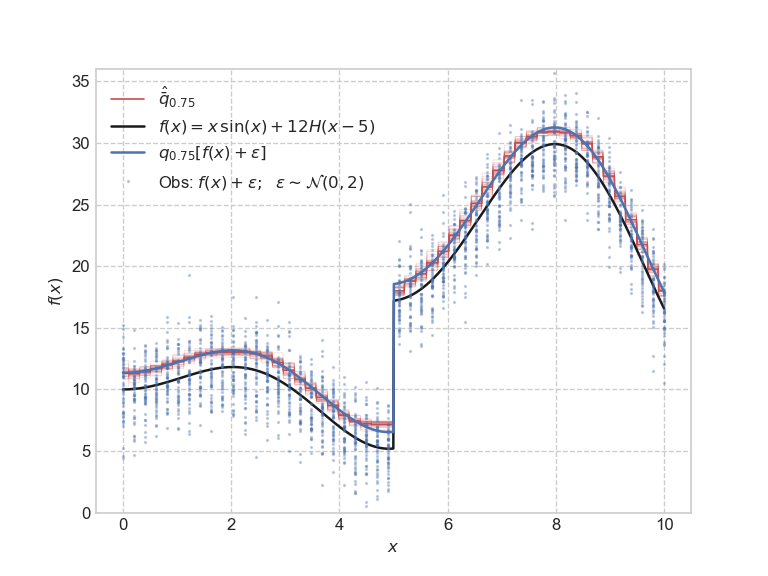
\includegraphics[width=0.53\linewidth]{figs/grad_boost/1d_boosted_regression_quantile_ex_0_75} }}\hspace*{-1.0em}%
    \subfloat[$\tau = 0.95$.]{{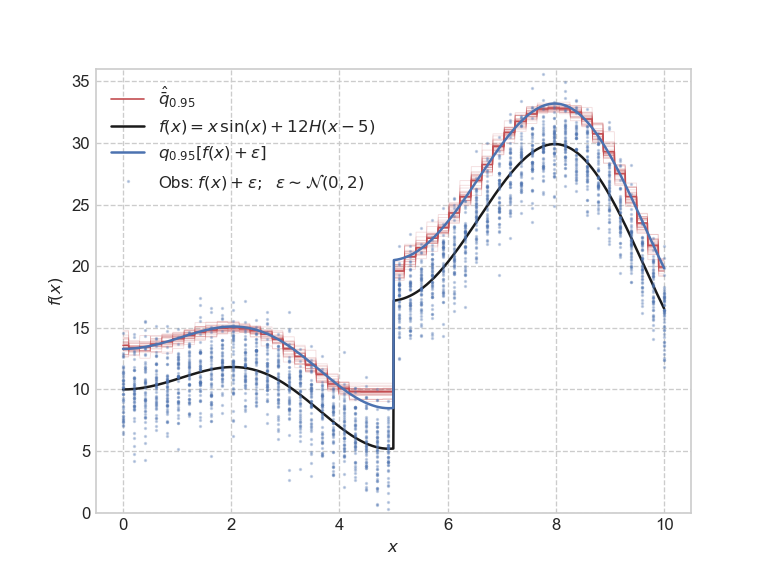
\includegraphics[width=0.53\linewidth]{figs/grad_boost/1d_boosted_regression_quantile_ex_0_95} }}\hspace*{-1.0em}%
    \caption[Gradient boosted quantile regression example.]{Gradient boosted quantile regression example.}%
    \label{fig:gb1}%
\end{figure}

Two candidate gradient boosting implementations were evaluated for use in this work.  A test problem was constructed to check that the standard gradient boosting regression technique is resilient to discontinuities in the data since the response fields are expected to abruptly change when moving across a spacer grid.  The function $y = x \mathrm{sin}(x) +12 \mathcal H(x-5)+\varepsilon$ with $x\in [0,10]$ was used for testing.  $\mathcal H$ denotes the Heaviside function. Synthetic noise, $\varepsilon \sim \mathcal N(0,2)$, was applied to the piecewise smooth test function.   5000 total samples were drawn from the test function. The test data was spatially aggregated to 100 axial levels to mimic CTF axial grid spacing.  Four separate quantile regressors ($\tau = \{0.5, 0.75, 0.9, 0.95 \})$ were then fit to the data by algorithm \ref{alg:boosting}. The predicted quantiles, conditioned on $x$, were compared to the expected results, as shown in figure \ref{fig:gb1}. For this problem results from the scikit-learn gradient boosting implementation are compared to a custom boosting implementation, named $pCRTree$, developed specifically to solve the classification and quantile regression problems in this work.  The residuals provided figure \ref{fig:gb2} show that the custom implementation performs similarly to the well-tested scikit-learn implementation with both models agreeing with the theoretical large-sample quantile distributions provided by equation \ref{eq:theory_qdist_1}.

\begin{figure}[H]%
    \centering
    \subfloat[$\tau = 0.5$ model residuals.]{{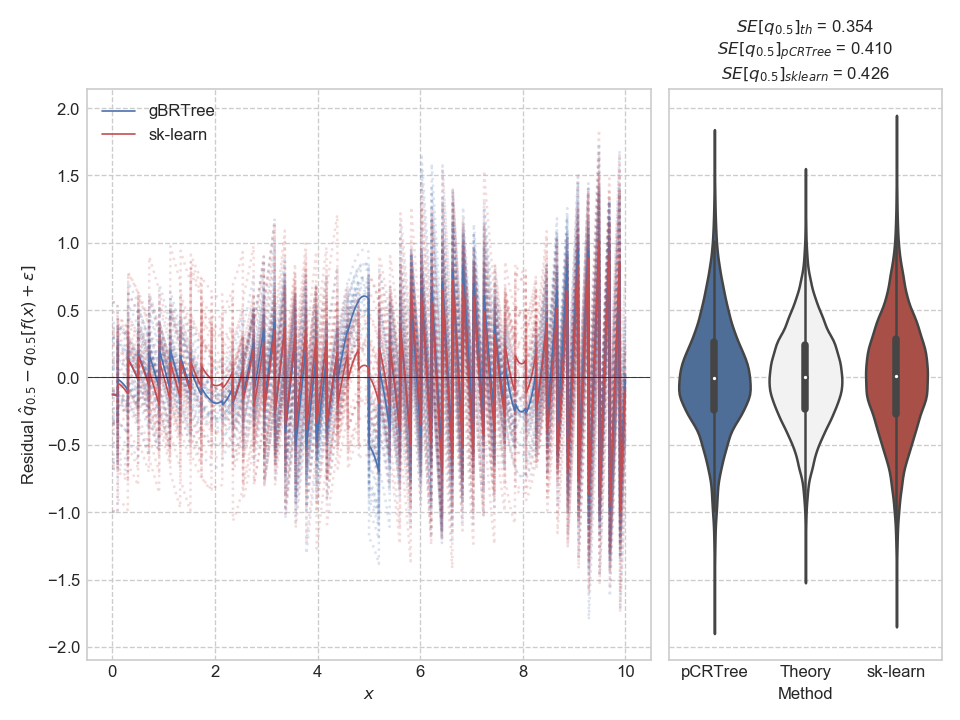
\includegraphics[width=0.53\linewidth]{figs/grad_boost/1d_boosted_regression_quantile_resid_0_5} }}\hspace*{-1.0em}%
    \subfloat[$\tau = 0.9$ model residuals.]{{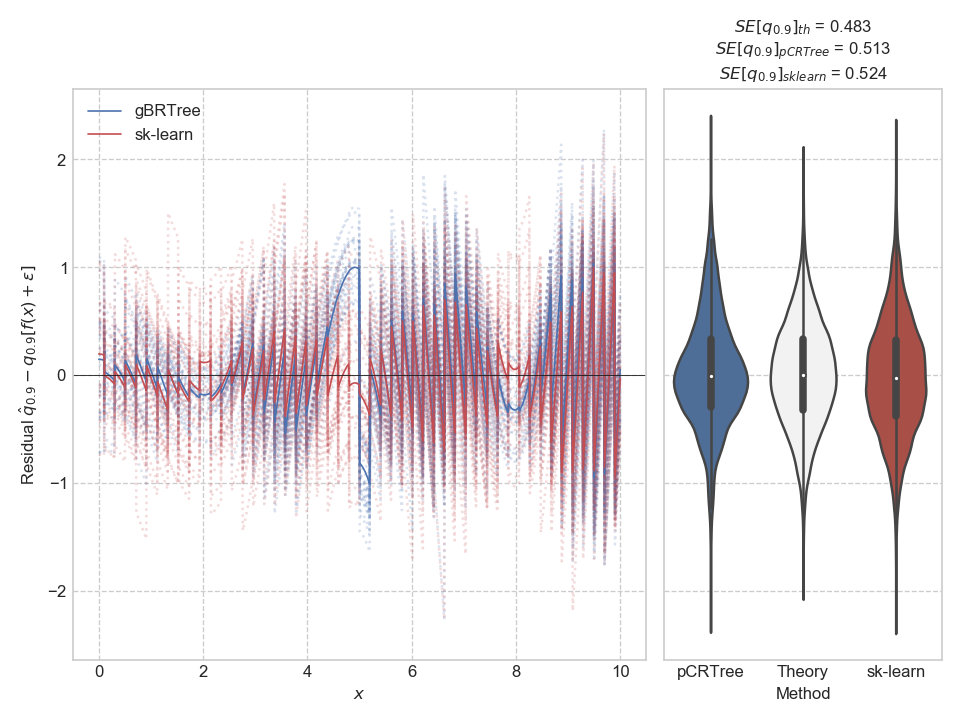
\includegraphics[width=0.53\linewidth]{figs/grad_boost/1d_boosted_regression_quantile_resid_0_9} }}\hspace*{-1.0em}%
    \\
    \subfloat[$\tau = 0.75$ model residuals.]{{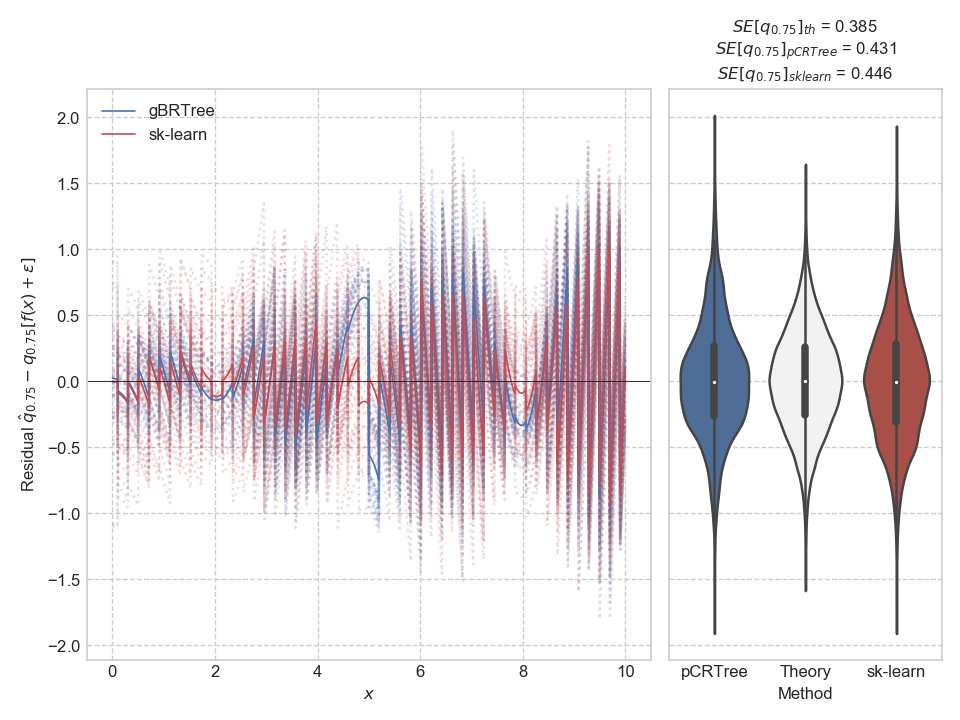
\includegraphics[width=0.53\linewidth]{figs/grad_boost/1d_boosted_regression_quantile_resid_0_75} }}\hspace*{-1.0em}%
    \subfloat[$\tau = 0.95$ model residuals.]{{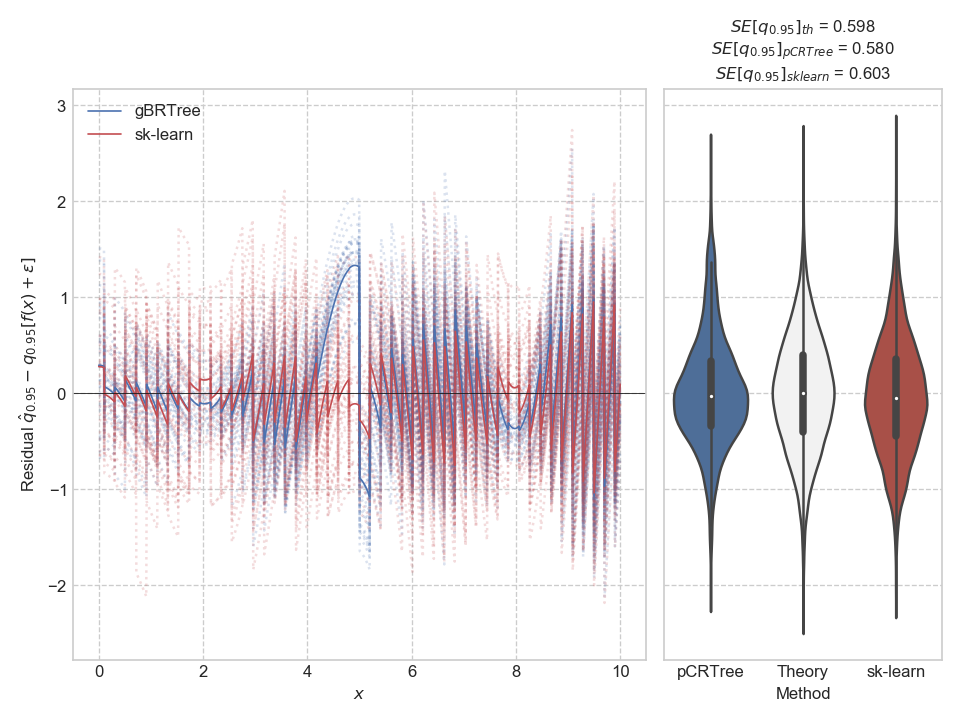
\includegraphics[width=0.53\linewidth]{figs/grad_boost/1d_boosted_regression_quantile_resid_0_95} }}\hspace*{-1.0em}%
    \caption[Gradient boosted quantile regression residual summary.]{Gradient boosted quantile regression residual summary.  The theoretical residual distribution were computed according to equation \ref{eq:theory_qdist_1}.} %
    \label{fig:gb2}%
\end{figure}

The parametric copula family which corresponds to a given set of local core conditions must also be determined in order to fully specify the copula required in the definition of the joint density function given in equation \ref{eq:simple_vine_model}.   This gives rise to a typical supervised classification problem which will be solved using the gradient boosting method.  The family of copula, $\mathbf \Theta_c$, i.e. either Frank, Clayton, or Gumbel, should be determined by the classifier provided a local core thermal hydraulic state vector $\mathbf p$.   The gradient boosted classification algorithm can be recovered by substituting the exponential loss function shown in equation \ref{eq:exploss} into algorithm \ref{alg:boosting}.   

\begin{align}
L(y, F(\mathbf p)) &= \E \left[ e^{-yF(\mathbf p)}\right] \nonumber \\
 &= \frac{1}{N}\sum_i^N e^{-y_iF(\mathbf p_i)}
\label{eq:exploss}
\end{align}
Where $y$ takes on integer values in $\{-1, 1\}$ for the classification problem.

A two-class test case was devised to validate the custom boosting implementation against the scikit-learn implementation.   This is meant as a demonstration for qualitative understanding of the boosted classification algorithm output.  In this problem red and blue points were emplaced in a two dimensional space as shown in figure \ref{fig:gb3}.  These predefined points form the necessary training data for the test problem. The goal of this test is to segregate the input space, $\{x, y\}$, into regions which are most likely to contain only one color of points. Results from the test 2-D classification test problem are shown in the figure.   In much the same way regression trees produce piecewise constant predictions, the boosted classifier partitions the input space by segregating the space along orthogonal splits.  

Classifier predictions are made by tallying the weighted predictions of each constituent fitted classification weak learner (CART tree) in the boosted model.  By tallying the predictions of all trees in the model one can obtain a probability mass function over all possible classes.  The probability mass function is visualized in figure \ref{fig:gb3}(b) wherein the predicted probability of the ``blue'' class obtained from the fitted boosted model is shown. The most likely class at each requested point is taken as the output of the classification model.

\begin{figure}[H]%
    \centering
    \subfloat[Class predictions.]{{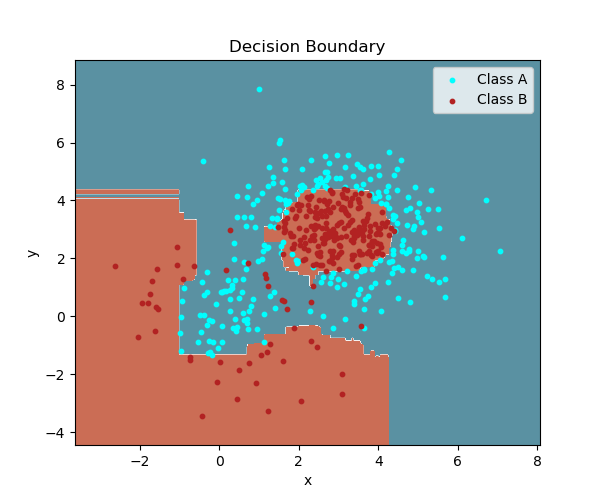
\includegraphics[width=0.50\linewidth]{figs/grad_boost/dblgauss_boosted_classify_ex} }}\hspace*{-1.0em}%
    \subfloat[Blue class probability.]{{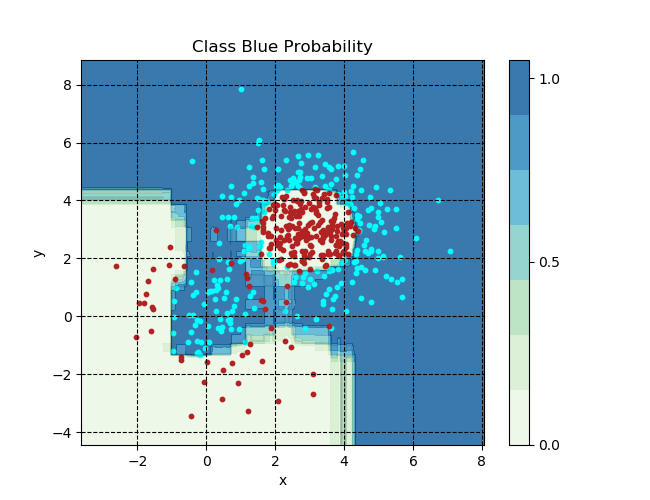
\includegraphics[width=0.54\linewidth]{figs/grad_boost/dblgauss_boosted_classify_probs} }}%
    \caption{Two-class gradient boosted classifier example.}%
    \label{fig:gb3}%
\end{figure}

Finally, gradient boosting can be used to estimate the relative explanatory power of each predictive variable included in the model.  This is done by tallying the number of times a particular dimension is split upon in the CART fitting process and weighting these splits by a gain measure.  The gain can be interpreted as the benefit of making a particular split in the decision tree as measured by improvement in $R^2$ for regression problems, or improvement in class purity as measured by the Gini impurity ratio for classification problems.  Finally, a weighted sum of the split gains of each tree is performed over all boosted iterations to obtain relative variable importances. Friedman provides a detailed explanation of this relative variable importance computation \cite{friedman2001}.  This ability of gradient boosting to identify important predictors has been exploited in email filter and web page ranking applications \cite{chapelle2011}, \cite{Tyree2011}.  In the case of copula prediction, exogenous variables which are extraneous can be detected and eliminated from the model to save computation time.  
%The ability to identify unimportant features is demonstrated in section \ref{sec:feature_eng} in figure \ref{fig:ktauregfeatureimp}.


\subsection{Monte Carlo Crud Estimation}
\label{chap:mc_crud}

Before applying a sampling procedure to the temperature and TKE surface fields on a given CTF face, the the joint density function is reconstructed from copula and marginal distributions.   On CTF face $j$, the gradient boosted model is queried for the conditional quantiles and the copula shape parameter:

\begin{align}
\hat \theta_j \leftarrow  & {\mathcal F_M}(\mathbf p_j, \mathbf z_j) \nonumber \\
 \hat \theta_j =& \{\hat \theta_{j,c}, \hat \theta_{j,\{T,k\}} \}
\end{align}
The CTF face index is dropped in the remainder of this section to reduce subindex clutter.

Provided estimates for the conditional quantiles, $\hat \theta_{\{T,k\}}$ in each face, the margins are defined by their quantile functions as shown in equation \ref{eq:cdf_from_qtau}.  After separate reconstruction of the margins and applying the boundary heat flux independence assumption shown previously in equation \ref{eq:simple_vine_model}, equation \ref{eq:joint_t_tke_q} defines the joint density.

\begin{equation}
h(T, k, q'') = f_T(T;\hat \theta_T) f_k(k;\hat \theta_k) f_{j,q''}
[ c_{T,k}(F_T(T;\hat \theta_{T})F_k(k;\hat \theta_{k});\hat \theta_c)]
\label{eq:joint_t_tke_q}
\end{equation}

After reconstruction of the joint temperature, boundary heat flux and turbulent kinetic energy distribution on each patch, the goal is to draw samples from the copula based distribution with arbitrary margins.  This is accomplished through the methods outlined by section \ref{sec:sampling_copula} in equation \ref{eq:h_inv_sample}.

With the ability to draw samples from a multivariate distribution now established, the Monte Carlo approximation of integral \ref{eq:expected_crud} follows and is represented by equation \ref{eq:mc_expected_crud}.  Let $X=\{T,k,q''\}$.
\index{Monte Carlo Sampling}

\begin{equation}
\E(\mathcal G(X)) \approx \frac{1}{N} \sum_i^N \mathcal G(X_i), \ \mathbf{X} \sim {h}
\label{eq:mc_expected_crud}
\end{equation}

Rather than sampling from the density function $h$, one may draw samples from an alternate proposal density distribution denoted, $\tilde h$, and appropriately weight the samples by the probability ratio of the original density to the proposal density, $h/\tilde h$, so to avoid introducing bias in the approximation of the expected value.  This leads to the importance sampling formulation of approximating integral \ref{eq:expected_crud}  which is given in equation \ref{eq:mc_imp_expected_crud}.

\begin{equation}
\E(\mathcal G(X)) \approx \frac{1}{N} \sum_i^N \mathcal G(X_i) \frac{h(X_i)}{\tilde h(X_i)}, \ \mathbf{X} \sim \tilde{h}
\label{eq:mc_imp_expected_crud}
\end{equation}
\index{Importance Sampling}
In principal the proposal distribution, $\tilde h$, may be radically different from the target density, $h$. In practice computing the optimal choice for the proposal density distribution is non-trivial. The generic original and proposal densities can be written simply as shown in equation \ref{eq:mc_imp_int_2}. 
%A method for determining a near optimal proposal distribution is provided in section \ref{sec:Importance Sampling}.

\begin{align}
    h(T, k, q'') &= c(F_T(T), F_k(k)) f_T f_k f_{j,q''}  \nonumber \\
    \tilde h(T, k, q'') &= \tilde c(\tilde F_T(T), \tilde F_k(k)) \tilde f_T \tilde f_k f_{j,q''}
\label{eq:mc_imp_int_2}
\end{align}

\begin{equation}
\E(\mathcal G(X)) \approx \frac{1}{N} \sum_i^N \mathcal G(X_i) \omega(X_i), \ \mathbf X \sim \tilde c(\tilde F_T(T), \tilde F_k(k)) \tilde f_T \tilde f_k f_{j,q''}
\label{eq:mc_imp_int2}
\end{equation}

with the probability ratio of the target density to the proposal given by \ref{eq:imp_prob_ratio}:

\begin{equation}
\omega_i = \frac{h_i}{\tilde h_i} = \frac{f_T(T_i) f_k(k_i)c(F_T(T), F_k(k))}
  {\tilde f_T(T_i) \tilde f_k(k_i) \tilde c(\tilde F_T(T), \tilde F_k(k))}
\label{eq:imp_prob_ratio}
\end{equation}

%In the case that the proposal and target copula densities are assumed to be the same equation \ref{eq:imp_prob_ratio} may be rewritten as \ref{eq:imp_prob_ratio2}.
%
%\begin{equation}
%\omega_i = \frac{f_1(x_i) f_2(x_i)}{\tilde f_1(x_i) \tilde f_2(x_i)}
%\label{eq:imp_prob_ratio2}
%\end{equation}
%
%In this work the target and proposal copula are taken to be the same function.

In some scenarios the proposal or target density is only known up to a constant, e.g. $h^* = c h(X)$.  In this case the probability ratio is known up to a constant of proportionality and requires renormalization:

\begin{equation}
\E(\mathcal G(X)) \approx \frac{ \sum_i^N \mathcal G_i(X) \omega_i(X)}{\sum_i^N \omega_i(x)}
,
 \ \mathbf X \sim \tilde c(\tilde F_T(T), \tilde F_k(k)) \tilde f_T \tilde f_k f_{j,q''}
\end{equation}

This is known as self normalizing importance sampling.  Traditional importance sampling may be applied in this case since $h$ and $\tilde{h}$ are properly normalized density functions in this hi2lo application which integrate to 1 over their respective support.


\section{Propagating Crud Through Time}

In the construction of the hi2lo method an assumption is made about the location of hot and cold spots on the rod surface as a function of time.   The presence of hot and cold spots downstream spacer grids and the location on the rod surface these spots occupy are assumed to be principally governed by the geometry of the mixing vanes and geometric layout of the fuel and guide tubes.  The influence of flow rate and core power on the relative location of the hot spots on the rod surface are assumed to be second order effects and are not explicitly captured by the hi2lo methodology at present.

\subsection{Hot Spot Stationarity}
\label{sec:hot_spot_stat}

The assumption that the location of eddy regions which develop downstream of spacer grids near the rod surface are principally governed by the grid geometry coupled with an assumption of steady state constant flow conditions leads to the notion of hot spot stationarity in time since the geometry of the core does not change throughout a cycle.  To achieve a stable location of hot and cold spots on the rod surface through time, the hi2lo methodology establishes a mapping from the sample space containing all possible outcomes of surface temperature and TKE sample pairs to a location on the rod surface.  To accomplish this, the order statistics of the joint temperate and turbulent kinetic energy distribution in each CTF patch are computed and the condition that the highest order statistic always falls on the same location within a given CTF patch is enforced.

Order statistics are well defined for a single dimensional random variable but in higher dimensions a consistent ordering is not possible.  Therefore, as shown in equation \ref{eq:weighting} a convex combination of the surface fields with user specified weights is used to reduce the random vector of T, TKE, and $q''$ samples on any given CTF patch into a univariate random variable denoted by $\mathbf{m}=\{m_0, m_1, ... m_N\}$.

\begin{equation}
    m_i = w_T \left( \frac{T_i - T_{min}}{T_{max} - T_{min}} \right) + w_k \left( \frac{k_i - k_{min}}{k_{max} - k_{min}} \right) +  w_q'' \left( \frac{q^{''}_i - q^{''}_{min}}{q_{max} - q_{min}} \right)
\label{eq:weighting}
\end{equation}
Where the sample remapping coefficients $\{w_T, w_k, w_{q''}\}$ are set at runtime by the hi2lo model user and sum to 1:
\begin{equation}
w_T + w_k + w_{q''} = 1
\end{equation}
Next the order statistics of $\mathbf m$ are computed such that $\mathbf m' = \{ m_{(0)} < m_{(1)}< ... m_{(N)} \}$.  As shown in figure \ref{fig:samplemapping}, the ordered samples are then emplaced on the CTF patch in an organized manner.  The sample space is denoted by $\Omega$ and a specific temperature, TKE, and boundary heat flux sample is denoted by $\mathcal F_i$ as a single dot residing inside the sample space.  The path taken on the patch surface is user controllable and is taken to be a simple serpentine left-to-right pattern in this work.
Typical values for the remapping coefficients are $w_T=0.6, w_k=0.4, w_{q''}=0$.  With this setting, relatively high temperate and low TKE samples are likely to remain in the same location on the rod surface over multiple resampling events.

\begin{figure}
    \centering
    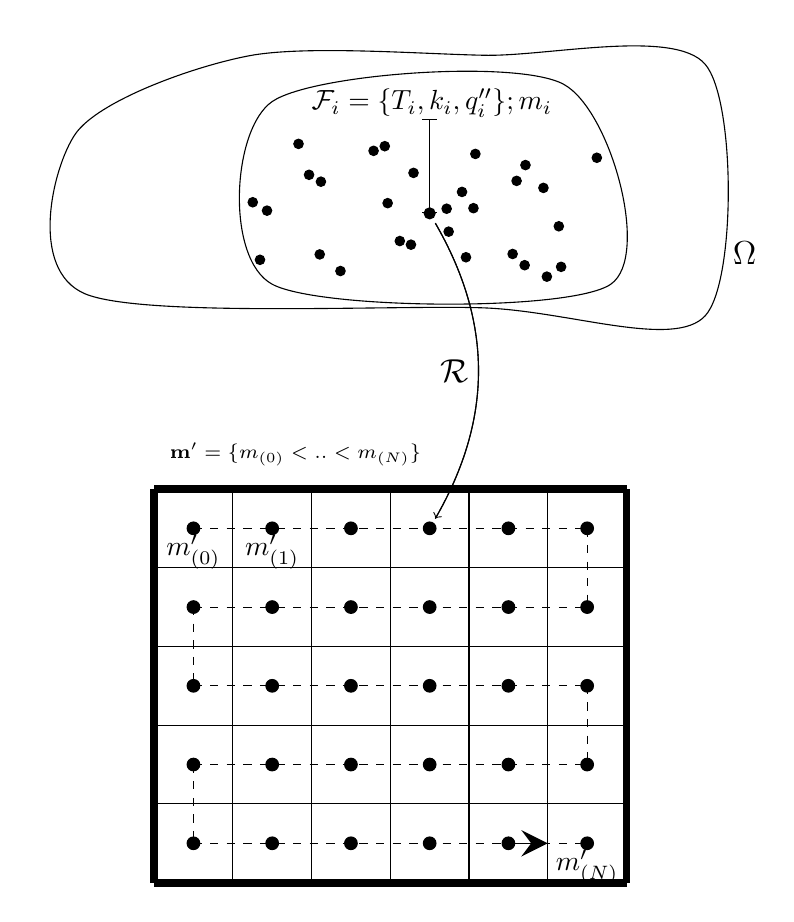
\begin{tikzpicture}
    \pgfmathsetseed{42}
    \pgfmathparse{0.5*rand}\let\r=\pgfmathresult
    \pgfmathparse{0.5*rand}\let\t=\pgfmathresult
% Sample space (blob)
\draw plot [smooth cycle] coordinates {(-1+\r,7.6-\r) (-1,9.8+\t) (1.2, 10.5) (4.2, 10.8+\t) (7,10.1-\t) (7,7.2) (4.3-\r, 7.3) } node at (7.5,8) {\large $\Omega$};
\draw plot [smooth cycle] coordinates {(1.5,7.6) (1.5,9.92) (5.2, 10.14) (5.8, 7.6) } ;
% Random samples
\foreach \u in {1,2,3,4,5,6,7,8,9,10,11,12,13,14,15,16,17,18,19,20,21,22,23,24,25,26,27,28,29}{
    \pgfmathparse{3.5+2.5*rand}\let\a=\pgfmathresult
    \pgfmathparse{8.5+0.9*rand}\let\z=\pgfmathresult
    \draw [fill=black] (\a, \z) circle (0.06cm);
}
\draw [fill=black] (3.5, 8.5) circle (0.07cm);
% Arrow map
\node (a) at (3.5, 8.5) {};
\node (b) at (3.5, 4.5) {};
\draw [->] (a) to [bend left] node [midway,left] {\large $\mathcal R$} (b);
\draw [decoration={markings,mark=at position 1 with
    {\arrow[scale=3,>=stealth]{>}}},postaction={decorate}] (a) to [bend left] (b);
% CTF face
\draw (0,0) grid (6,5);
\draw [line width=0.1cm] (0,0) -- (0,5);
\draw [line width=0.1cm] (0,0) -- (6,0);
\draw [line width=0.1cm] (6,0) -- (6,5);
\draw [line width=0.1cm] (0,5) -- (6,5);
% dots in grid
\foreach \x in {0.5,1.5,2.5,3.5,4.5,5.5} {
\foreach \a in {0.5,1.5,2.5,3.5,4.5}
{
    \draw [fill=black] (\x, \a) circle (0.08cm);
}
}
\fill (0.5,4.2) node {$m'_{(0)}$};
\fill (1.5,4.2) node {$m'_{(1)}$};
\fill (5.5,0.2) node {$m'_{(N)}$};
\foreach \c in {0.5,1.5,2.5,3.5,4.5}{
    \draw [dashed] (0.5,\c) -- (5.5, \c);
}
% draw serp path
\draw [dashed] (5.5, 4.5) -- (5.5, 3.5);
\draw [dashed] (5.5, 2.5) -- (5.5, 1.5);
\draw [dashed] (0.5, 3.5) -- (0.5, 2.5);
\draw [dashed] (0.5, 1.5) -- (0.5, 0.5);
\draw [decoration={markings,mark=at position 1 with
    {\arrow[scale=3,>=stealth]{>}}},postaction={decorate}] (4.5,0.5) -- (5,0.5);
% figure text
\node[text width=4cm] at (2.2,5.44) {\scriptsize $\mathbf m'=\{ m_{(0)}<..< m_{(N)} \}$};
\node[text width=5cm] at (4.5,9.9) {$\mathcal F_i=\{T_i, k_i, q''_i\}; m_i$};
\draw [|-|] (3.5, 8.5) -- (3.5, 9.7);
    \end{tikzpicture}
    \caption{Sample remapping.  A single CTF face is shown as the bold square with a grid overlay partitioning the patch surface.  In this figure the number of samples per CTF face is $N=30$.}
    \label{fig:samplemapping}
\end{figure}

Since the crud simulation package utilized in this work is one-dimensional, the pattern chosen for sample emplacement has no influence on the integrated crud result over a patch.  This would not be the case if the crud simulation package modeled a fully 3-D crud layer as the state of the neighboring crud nodes in that case would matter.  Interestingly, since the hi2lo model user specifies the sample remapping pattern at run time, a physically realistic pattern could be prescribed on the rod surface - even prescribed as a function of local core conditions leading to a hybrid strategy between the current pure statistical hi2lo procedure and the spatial remapping procedure implemented by Salko et. al \cite{salko17}.

\subsection{Time Stepping Scheme}
\label{sec:time_step_scheme}

Propagating the importance weights through discrete resampling steps requires special attention to ensure bias is not introduced into the crud results when moving through multiple time steps and VERA states.  The key observation is that the importance weights computed at a given resampling event should neither be double-counted nor discarded in subsequent resampling steps.  Instead, the importance weights are time averaged to achieve the correct importance weights used to evaluate the total crud mass on the rod surface at any given time step (resampling step).

Figure \ref{fig:stepscheme} depicts the time stepping scheme for a single patch. The patch index is not shown to reduce visual clutter. The VERA state-point index is denoted by $\ell$.  At the beginning of each VERA state-point the power distribution and thermal hydraulic conditions in the core change.  Here it is assumed there is a constant power profile and constant flow conditions over a VERA depletion step.

In figure \ref{fig:stepscheme} dotted arrows represent sampling from a probability distribution.  $\mathcal R$ is the spatial reordering map from sample space to a position on the rod surface. $\mathcal G$ represents the crud generation function provided by the crud simulation package which takes thermal hydraulic boundary conditions as input in addition to the previous crud state and produces a new crud state.  Resampling events are performed at time intervals $\Delta t_s$ and this interval is set at runtime by the user. 
%The influence of the resampling interval size is discussed in section \ref{sec:resample_freq_study}. 
The resample index is denoted by $s$.  The subscript, $(\cdot)_s$ , denotes evaluation at a resampling event.  A prime-notated variable,  $(\cdot)'$, represents a spatially re-mapped sample as in figure \ref{fig:samplemapping}.  At each resampling event the temperature, TKE and boundary heat flux samples are independently drawn from the reconstructed joint probability $\hat H^\ell$.  Assume that the resample time step is constant and equal to $\Delta t_s$.

\begin{figure}
\centering
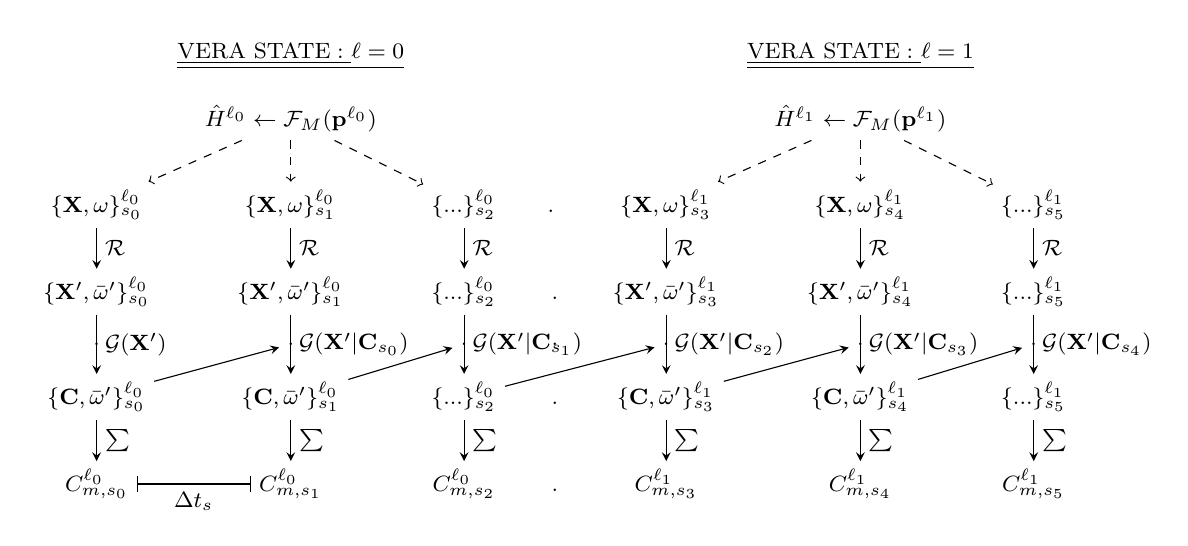
\begin{tikzpicture}
\footnotesize
\matrix (m) [matrix of math nodes,row sep=0.9em,column sep=0.5em,minimum width=0.5em]
  {
      & \underline{\mathrm{\underline{VERA\ STATE:\ }} \ell = 0} & & & & \underline{\mathrm{\underline{VERA\ STATE:\ }} \ell = 1} & & \\  %m-1
      & \hat H^{\ell_0}_{} \leftarrow \mathcal F_M(\mathbf p^{\ell_0}) & & & & \hat H^{\ell_1 }_{} \leftarrow \mathcal F_M(\mathbf p^{\ell_1}) & & \\  %m-2
      & & &\\  %m-3
    \{\mathbf X, \omega \}^{\ell_0}_{s_0} & \{\mathbf X, \omega \}^{\ell_0}_{s_1} & \{...\}^{\ell_0}_{s_2} & \ \ \ .\ \ \ \  & \{\mathbf X, \omega \}^{\ell_1}_{s_3} & \{\mathbf X, \omega \}^{\ell_1}_{s_4} & \{...\}^{\ell_1}_{s_5} \\ %m-4
                           &\\ %m-5
    \{\mathbf X', \bar \omega' \}^{\ell_0}_{s_0} & \{\mathbf X', \bar \omega' \}^{\ell_0}_{s_1} & \{...\}^{\ell_0}_{s_2}  & . &  \{\mathbf X', \bar \omega' \}^{\ell_1}_{s_3} & \{\mathbf X', \bar \omega' \}^{\ell_1}_{s_4} & \{...\}^{\ell_1}_{s_5} \\ %m-6
     . & . & . & . & . & . & . &  \\ %m-7
    \{\mathbf C, \bar \omega' \}^{\ell_0}_{s_0} & \{\mathbf C, \bar \omega' \}^{\ell_0}_{s_1} & \{...\}^{\ell_0}_{s_2} &  . &  \{\mathbf C, \bar \omega' \}^{\ell_1}_{s_3} & \{\mathbf C, \bar \omega' \}^{\ell_1}_{s_4} & \{...\}^{\ell_1}_{s_5} \\ %m-8
                           &\\ %m-9
    C_{m,s_0}^{\ell_0} & C_{m,s_1}^{\ell_0} & C_{m,s_2}^{\ell_0} & . &  C_{m,s_3}^{\ell_1}  & C_{m,s_4}^{\ell_1} & C_{m,s_5}^{\ell_1} \\ %m-10
  };
  \path[-stealth]
  (m-10-1) edge [solid,|-|] node [below]{$\Delta t_s$} (m-10-2)
  (m-2-2) edge [dashed,->] (m-4-1)
          edge [dashed,->] (m-4-2)
          edge [dashed,->] (m-4-3)
   (m-2-6) edge [dashed,->] (m-4-5)
           edge [dashed,->] (m-4-6)
           edge [dashed,->] (m-4-7)
  % vert linkages
          (m-4-1) edge node [right] {$\mathcal R$} (m-6-1)
          (m-4-2) edge node [right] {$\mathcal R$} (m-6-2)
          (m-4-3) edge node [right] {$\mathcal R$} (m-6-3)
           (m-4-5) edge node [right] {$\mathcal R$} (m-6-5)
           (m-4-6) edge node [right] {$\mathcal R$} (m-6-6)
           (m-4-7) edge node [right] {$\mathcal R$} (m-6-7)
  %
          (m-6-1) edge node [right] {$\mathcal G(\mathbf X')$} (m-8-1)
          (m-6-2) edge node [right] {$\mathcal G(\mathbf X'|\mathbf C_{s_0})$} (m-8-2)
          (m-6-3) edge node [right] {$\mathcal G(\mathbf X'|\mathbf C_{s_1})$} (m-8-3)
           (m-6-5) edge node [right] {$\mathcal G(\mathbf X'|\mathbf C_{s_2})$} (m-8-5)
           (m-6-6) edge node [right] {$\mathcal G(\mathbf X'|\mathbf C_{s_3})$} (m-8-6)
           (m-6-7) edge node [right] {$\mathcal G(\mathbf X'|\mathbf C_{s_4})$} (m-8-7)
  %
          (m-8-1) edge node [right] {$\sum$} (m-10-1)
          (m-8-2) edge node [right] {$\sum$} (m-10-2)
          (m-8-3) edge node [right] {$\sum$} (m-10-3)
           (m-8-5) edge node [right] {$\sum$} (m-10-5)
           (m-8-6) edge node [right] {$\sum$} (m-10-6)
           (m-8-7) edge node [right] {$\sum$} (m-10-7)
  % diag linkages
          (m-8-1) edge (m-7-2)
          (m-8-2) edge (m-7-3)
          (m-8-3) edge (m-7-5)
            (m-8-5) edge (m-7-6)
            (m-8-6) edge (m-7-7);
\end{tikzpicture}
\caption{Multi-state point time stepping overview. Dashed arrows represent sampling from a distribution.  Solid arrows represent a functional mapping or operation.}
\label{fig:stepscheme}
\end{figure}

A dependency in time is introduced by the crud growth step because the current crud growth rate depends on the previous crud state (e.g. a severely thick crud deposit will behave differently than a small crud deposit).  This time dependence is denoted by the diagonal arrows linking the crud states together across resampling events in figure \ref{fig:stepscheme}.

Since the resampling time step size is constant the time corresponding to any given sample event is computed by multiplying the resampling event index by the constant resampling step size:
\begin{equation}
t_{s_n} = n\Delta t_s
\end{equation}

The time averaged sample weights are in general updated by equation \ref{eq:time_sample_weights1} at each resampling step.
Recall that the ratio of the target density and the sampling distribution density is denoted by $\omega$ and is given in equation \ref{eq:imp_prob_ratio}.

\begin{equation}
\bar \omega'_{{s_n},i} =
\left( \frac{\sum_{l}^{n-1} \Delta t_{s_l}}{\sum_l^n \Delta t_{s_l}} \right) \bar \omega'_{n-1,i} +
\left( \frac{\Delta t_{s_n}}{\sum_l^n \Delta t_{s_l}} \right) \omega'_{n,i}
\label{eq:time_sample_weights1}
\end{equation}
Where $i$ is the sample index within a single CTF face.

After applying the constant resample step size assumption the time averaged sample weights are updated at each resampling step according to equation \ref{eq:time_sample_weights3}.

\begin{align}
\bar \omega'_{{s_n},i} &= \left( \frac{(n-1) \Delta t_s}{n \Delta t_s} \right) \bar \omega'_{n-1,i} + \left( \frac{\Delta t_s}{n \Delta t_s} \right) \omega'_{n,i} \nonumber \\
 &= \left( \frac{(n-1)}{n} \right) \bar \omega'_{n-1,i} + \left( \frac{1}{n} \right) \omega'_{n,i}
\label{eq:time_sample_weights3}
\end{align}

After each resampling event the total crud mass, $C_m$ on a CTF face, is computed by a wighted sum given in equation \ref{eq:patch_sum_mass}.  The sampling and weighting procedure is depicted in figure \ref{fig:crudsamplesdt}.

\begin{equation}
C_{m} = \left(\frac{A}{\sum_i^N \bar \omega'_i}\right) \sum_i^N C'_i \bar \omega'_i
\label{eq:patch_sum_mass}
\end{equation}
Where $N$ is the number of samples drawn per CTF face and $A$ is the surface area of the $j^{th}$ CTF face.  The re-stepping index $n$ and the patch index $j$ are dropped to reduce clutter in equation \ref{eq:patch_sum_mass}.

The crud stepping strategy is explicit in time as the next crud samples are drawn from knowledge of the previous crud state and the current thermal hydraulic conditions.  Feedback between the crud state and the underlying density functions are not captured in the hi2lo stepping scheme.  The presence of crud influences the rod surface temperature distribution due to two competing effects: Providing favorable conditions for bubble nucleation and an increased thermal resistance.  Though these effects are slight they impact not only the mean rod surface temperature but also higher moments about the mean of the probability densities of surface temperature.  These higher order feedbacks are not currently considered, however it is possible to incorporate the current crud state into the explanatory variable set used by the machine learning model to resolve this feedback between the crud thickness and the higher order moments of temperature and TKE about the CTF prediction.  This remains as future work as the impact of the crud layer on the flow field is hypothesized to only significantly matter if the crud deposits significantly shifts the locations of the onset of nucleate boiling within the core.

\begin{figure}[H]
    \centering
    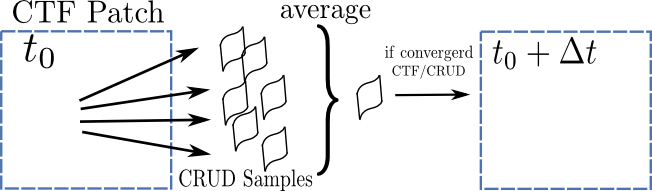
\includegraphics[width=0.6\linewidth]{figs/theory/crud_samples_dt}
    \caption[Time step procedure depicted for a single CTF face]{Time step procedure depicted for a single CTF face.  A single resampling event is shown.}
    \label{fig:crudsamplesdt}
\end{figure}

\section{Method Summary}

The time stepping, importance sampling and surface sample remapping strategies may be included into algorithm \ref{algo:basic_crud_algo} to provide a detailed overview of the hi2lo procedure.  The expanded version of the hi2lo model is given in algorithm \ref{algo:hi2lo_crud_algo}.

Algorithm \ref{algo:hi2lo_crud_algo} begins with the same pre-processing and machine learning procedure outlined in the generic hi2lo algorithm \ref{algo:basic_crud_algo}.  \emph{Lines 2-5:} 
%An overview of the CFD data pre-processing procedure is given in section \ref{sec:preprocessing} and the gradient boosted quantile regression model fitting routine is discussed in section \ref{chap:GBRT}.
\emph{Line 9:} Reconstructs the temperature and TKE CDFs from quantiles.  The details of reconstructing a cumulative density function using a set of predicted quantiles was discussed in section \ref{chap:quantiles}.  \emph{Line 10:} The simplified treatment of the boundary heat flux distribution was discussed in section \ref{sec:dep_structure} and the application of this simplification resulted in a compact representation of the joint distribution of temperature, TKE, and BHF in each CTF face given in equation \ref{eq:simple_vine_model}.   \emph{Lines 15-16:} Involves the construction of the importance sampling distributions.  
%The details of this procedure are given in section \ref{sec:Importance Sampling}. 
\emph{Line 17-18:} Draws samples from the reconstructed joint distribution and follows the standard importance sampling procedure outlined in section \ref{chap:mc_crud}.  \emph{Line 19:} Performs the spatial remapping procedure required to preserve hot spot stationarity.  The details of this procedure may be found in section \ref{sec:hot_spot_stat}.  \emph{Line 20:} The importance weights are time averaged according to method provided in section \ref{sec:time_step_scheme} before the the crud distribution is integrated in each CTF face at each resampling step.

\begin{algorithm}[H]
    \captionsetup{labelfont={sc,bf}, labelsep=newline}
    \caption{Statistically based hi2lo method for time dependent crud prediction.}
    \begin{algorithmic}[1]
        \STATE \textbf{Initialization}
        \STATE (1) Pre-process training set.
        \STATE $\ \ $   (1b) Fit the joint distribution parameters to known CFD data: $\theta(\mathbf p, \mathbf z)$.
        \STATE $\ \ $   (1c) \textbf{def:}  $\ \theta \leftarrow \mathcal F_M(\mathbf p, \mathbf z)$
        \STATE (2) Train model:  $\hat{\mathcal F_M} =  \mathrm{argmin}_{\mathcal F}$
        $\E \left[ L(\mathcal{F}_M (\mathbf p, \mathbf z), \theta(\mathbf p, \mathbf z)) \right] $
        \FOR {VERA State, $v$}
        \FOR {CTF face, $j$}
          \STATE Evaluate ML model $\hat \theta_j \leftarrow \hat{\mathcal F_M}(\mathbf p_j, \mathbf z_j)$ \\
          $\ \ \hat \theta_j = \{\hat \theta_{j,c}, \hat \theta_{j,\{T,k\} }$
          \STATE Reconstruct margins (CDFs) from quantiles  \\
          $\ \ \hat F_{j,T}= Q^{-1}(T; \{\hat{\theta}_{j,\{T,k\} } \})$ , $\hat F_{j,k}= Q^{-1}(k; \{\hat{\theta}_{j,\{T,k\} } \})$
          \STATE Def $q''$ margin  $f_{j,q''} = \delta_{(q''_\mathrm{j,ctf})}$
          \STATE Reconstruct joint distribution $\hat h_j(\cdot |\hat \theta_j) = \hat f_{j,T} \hat f_{j,k} f_{j,q''} c(\hat F_{j,T}, \hat F_{j,k}; \hat \theta_{j,c})$ \;
        \ENDFOR
          \FOR {Resample time step, $s,\ \Delta t_s$}
            \FOR {CTF face, $j$}
            \STATE Def importance  mixture quantile functions by equation %\ref{eq:imp_mix_dists} \\
                $\ \ \tilde Q_{j,k} = \lambda_{0,k} \hat Q_{j,k}  + \lambda_{1,k} Q_{\beta_k}(k; \vartheta_k)$,
                $\ \ \tilde Q_{j,T} = \lambda_{0,T} \hat Q_{j,T}  + \lambda_{1,T} Q_{\beta_T}(T; \vartheta_T); $ \\
                $\ \ \sum_i \lambda_i = 1, \ \ \tilde F_{j,T} = \tilde Q^{-1}_{j,T},\ \  \tilde F_{j,k} = \tilde Q^{-1}_{j,k} $
              \STATE Def importance sampling distribution $\tilde h_j = \tilde f_{j,T} \tilde f_{j,k} c(\tilde F_{j,T}, \tilde F_{j,k}; \hat \theta_{j,c}) $
              \STATE Draw samples $\mathbf x \sim \tilde h_j$ \;
              \STATE Compute importance weights $\omega = \hat h_j(\mathbf x) /  \tilde h_j(\mathbf x) $
              \STATE Re-map samples  $\mathbf x', \omega' \xleftarrow[\text{ }]{\mathcal R} \mathbf x, \omega $
              \STATE Update importance weights by equation \ref{eq:time_sample_weights3}
              \STATE Evaluate equation \ref{eq:expected_crud} via importance sampling \\
                $\ \ \mathbf C_s = \mathcal G(x'_i; \mathbf C_{s-1}, \mathbf I, \Delta t_s)$ \\
              \STATE Crud mass at step $s$ in patch $j$:
                $\ \ C_{s,j,m} = \left( \frac{A_j}{\sum_i^N \bar \omega'_i} \right) \sum_i^N C_{s,i,j,m} \bar \omega'_i$
          \ENDFOR
        \ENDFOR
        \ENDFOR
    \end{algorithmic}
    \label{algo:hi2lo_crud_algo}
\end{algorithm}

All model variables which are set at runtime are provided in table \ref{tab:hi2lo_params}.  Recommended settings are also provided by each model parameter.

\begin{table}[H]
    \begin{center}
        \caption[Runtime model parameters.]{Runtime hi2lo model parameters.}
        \begin{tabular}[h]{|l | l | L | }
            \hline
            Sym & Default Value & Purpose  \\
            \hline
            \hline
            $\Delta t_s$ & 25 $[days]$ &  Resampling time step size. \\
            \hline
            $N$ & 400 & Number of samples drawn per CTF face. \\
            \hline
            $N_{Q_{k}}$ & 20 & Number of quantiles used in TKE marginal distribution reconstruction. \\
            \hline
            $N_{Q_{T}}$  & 20 & Number of quantiles used in temperature marginal distribution reconstruction. \\
            \hline
            $w_k$  & 0.6 & TKE weighting factor used to remap samples on the rod surface. \\
            \hline
            $w_T$  & 0.4 & Temperature weighting factor used to remap samples on the rod surface. \\
            \hline
            $\vartheta_T$  & $\{1.0, 0.9 \}$ & Beta distribution parameters for temperature importance distribution. \\
            \hline
            $\vartheta_k$  & $\{1.1, 1.2 \}$ & Beta distribution parameters for TKE importance distribution. \\
            \hline
            $\lambda_{0,T},\lambda_{1,T}$  & $\{0.6, 0.4 \}$ & Mixture weighting parameters for temperature importance distribution. \\
            \hline
            $\lambda_{0,k},\lambda_{1,k}$  & $\{0.7, 0.3 \}$ & Mixture weighting parameters for TKE importance distribution. \\
            \hline
            \hline
            $b_m$  & 4  & Gradient boosting model parameter: Max CART tree depth.  A larger CART tree depth value improves the quality of fit of each weak-learner but increases overfitting. \\
            \hline
            $\nu$ & 0.01  & Gradient boosting model parameter:  Learning rate. \\
            \hline
            $M$  & 4000 & Gradient boosting model parameter:  Number of boosted iterations. \\
            \hline
        \end{tabular}
        \label{tab:hi2lo_params}
    \end{center}
\end{table}

Finally, the simplifications and assumptions made in the construction of the hi2lo model are reviewed.  The model requires that within a CTF face no spatial information is retained.  The crud simulation package, MAMBA, used in this work is a one-dimensional code and therefore this simplification has no influence on the integrated crud results within each CTF face.  The boundary heat flux is treated independently from the rod surface temperature or TKE.  This simplifies the copula model used to reconstruct the joint distribution in each face.  Hot spots are assumed to remain stationary on the rods' surface as a function of time.  This assumption can be slightly relaxed with tuning of the sample remapping procedure; however, this assumption simplifies the treatment of the time dependent nature of crud build up in the core.  The assumption takes into account that as time marches forward, the rate of crud growth depends on the previous crud state.  The viability of these assumptions will be investigated in the following sections.  The aim of the hi2lo model is to reproduce gold standard crud results provided by high fidelity CFD coupled crud simulations.  The application of the simplifications should not impede the ability of the model to reproduce the correct axial and total crud deposition on the rod surface.


\appendices
\chapter{Rod Surface Heat Transfer}
\label{chap:app_d}
%! TEX root = ../outline.tex
% ------------------------- TH definitions ----------------------- %
\section{Subcooled Boiling and DNB}

The relationship between the surface temperature of an internally heated object and the heat flux from the surface into the surrounding fluid is shown in figure \ref{fig:boiling_curve}.

\begin{figure}[H]
    \centering
    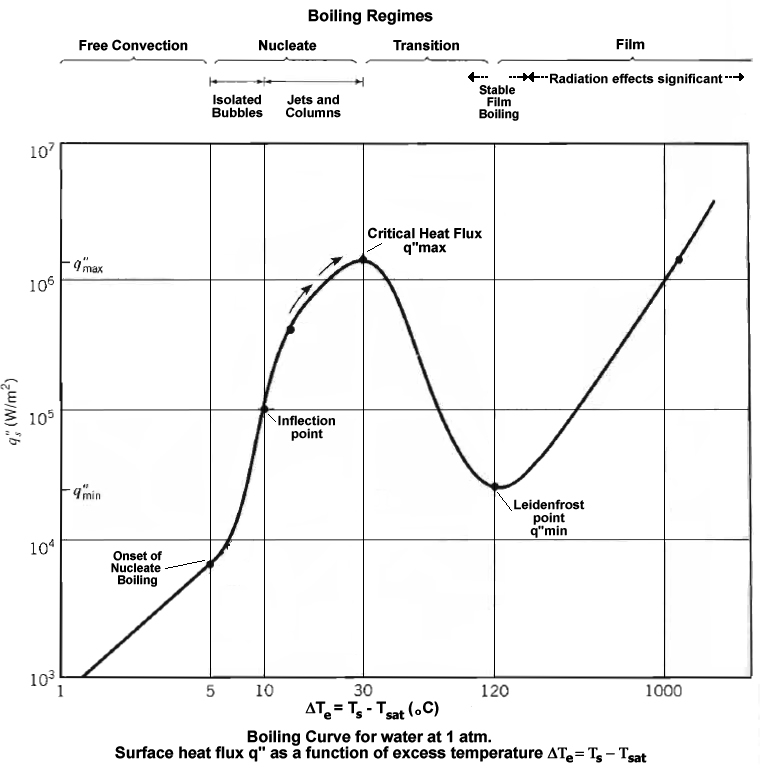
\includegraphics[width=0.7\linewidth]{../proposal/images/boiling_curve}
    \caption{Boiling curve.}
    \label{fig:boiling_curve}
\end{figure}


The curve can be approximated by equation \ref{eq:boil_h}.  Note that surface temperature $T_s$ is equivalent to the wall temperature $T_w$ in the equations which follow.
The critical heat flux (CHF) is the point at which film boiling begins to dominate and is accompanied by a precipitous drop in the heat transfer and a rise in the surface temperature.  This condition is known as departure from nucleate boiling (DNB) and must be avoided when operating a PWR.
\index{Departure from Nucleate Boiling}

\begin{equation}
q''(T_w) = 
\begin{cases}
      h(T_w-T_{\infty}), & \mbox{if } T_w < T_{sat} \\
      h(T_w-T_{\infty}) + q''_{nb} ,  & \mbox{if } T_{sat} \leq T_w < T_{CHF} 
\end{cases}
\label{eq:boil_h}
\end{equation}
Where $h$ is the single phase convective heat transfer coefficient which is in turn a function of the Nusselt number given in equations \ref{eq:htc} and \ref{eq:db}.  The contribution of nucleate boiling to the heat transfer can be approximated by the Rohsenow model given in \ref{eq:ros} \cite{rohsenow51}.

\begin{equation}
q''_{nb} = {{\mu }_{L}}{{h}_{fg}}{{\left[ \frac{g\left( {{\rho }_{L}}-{{\rho }_{v}} \right)}{\sigma } \right]}^{{}^{1}\!\!\diagup\!\!{}_{2}\;}}{{\left[ \frac{{{c}_{pL}}\left( {{T}_{w}}-{{T}_{sat}} \right)}{{{C}_{sf}}{{h}_{fg}}Pr_{L}^{n}} \right]}^{3}\;}
\label{eq:ros}
\end{equation}
Where $h_{fg}$ is the latent heat of vaporization, $\mu_L$ is the liquid viscosity, $\rho_v,\ \rho_L$ are the vapor and liquid phase densities, ${c}_{pL}$ is the specific heat of the liquid phase, and ${C}_{sf}$ is a tunable empirical constant.

\begin{equation}
h = \frac{k_l \mathrm{Nu}}{L} = \frac{q''}{T_w-T_{\infty}}
\label{eq:htc}
\end{equation}
Where $k_l$ is the thermal conductivity of the liquid, $L$ is the characteristic length scale, and $Nu$ is the Nusselt number.  For non-boiling flows over a flat vertical surface, the Nusselt number can be approximated by the
Dittus-Boelter equation:

\begin{equation}
\mathrm{Nu} = 0.023\, \mathrm{Re}^{4/5}\, \mathrm{Pr}^{n}
\label{eq:db}
\end{equation} 
\index{Dittus-Boelter}
Where $\mathrm{Re}$ is the Reynolds number and $\mathrm{Pr}$ is the Prandtl number.  $n$ is an empirically derived constant and is typically 0.4 for a heated flow.


\printindex

%! TEX root = ../dissertation_gurecky.tex

% \section*{References}
\newpage


\bibliographystyle{unsrt}
\bibliography{sections/refs}
% \addcontentsline{toc}{chapter}{Bibliography}



\end{document}